\documentclass[
	ngerman,	%deutsch
	a4paper,	%A4 Format
	12pt,		%Schriftgr��e
	oneside,		%einseitig
%	liststoto
%	bibtotocnumbered
				]{article}%Artikel
\usepackage[ansinew]{inputenc}	%Zeichenkodierung
\usepackage[T1]{fontenc}
\usepackage[english]{babel}			%deutsche Silbentrennung
\usepackage[english]{hyperref}
%\usepackage[sort&compress]{natbib}
\usepackage{
    textcomp,
	amsmath,
	amssymb,
    libertine,
	amsfonts,		%Mathepakete
    graphicx,		%Bilder einbinden
	a4wide,			%volle Seitenbreite
	multirow,		%Zellen verbinden in Tabellen
	booktabs,		%sch�ne Tabellen
	array,			%Arrays halt
	float,			%Gleitumgebungen genau HIER setzen
	caption,		%zus�tzliche Optionen f�r Unterschriften
	fancyhdr,		%sch�ne Kopf-/Fu�zeilen
	ragged2e,		%besseres Centering, RaggedRight und RaggedLeft
	caption,
	hhline,
	wrapfig,
    listings,
    bm
	}
\usepackage[toc,page]{appendix}

%Spalten mit Breitenangabe und Umbr�chen
\newcolumntype{C}[1]{>{\centering\arraybackslash}p{#1}} 	% zentriert
\newcolumntype{R}[1]{>{\raggedleft\arraybackslash}p{#1}} 	% linksb�ndig
\newcolumntype{L}[1]{>{\raggedright\arraybackslash}p{#1}} 	% rechtsb�ndig

%andere Bezeichnung f�r Abbildungen und Tabellen
\addto\captionsngerman{%
%  \renewcommand{\figurename}{Abb.}
%  \renewcommand{\tablename}{Tab.}
}


%Def vom Absatz
\newcommand{\absatz}{\hfill \medskip \newline}

%Def von der Einheit
\newcommand{\ein}{\ensuremath{\,\mathrm}}

%nice dirac brackets
\newcommand{\ket}[1]{\left| #1 \right>} % for Dirac bras
\newcommand{\bra}[1]{\left< #1 \right|} % for Dirac kets
\newcommand{\braket}[2]{\left< #1 \vphantom{#2} \right| \left. #2 \vphantom{#1} \right>} % for Dirac brackets

\newcommand{\vect}[1]{\boldsymbol{\mathbf{#1}}}



%adjust nested math sizes
%\DeclareMathSizes{12}{12}{8}{8}

%Papiergeometrie
\setlength{\headheight}{40pt}
\setlength{\textheight}{0.75\paperheight}
\setlength{\parindent}{0px}
\setlength{\parskip}{0,1em}
\setlength{\topmargin}{-10mm}

%Kopf- unf Fu�zeilen
\pagestyle{fancy}
\fancyhf{}
\fancyhf[LH]{\textsc{Progress Report}}
\fancyhf[RH]{\small{Jakob Kolb}}
\fancyhf[CF]{\thepage}
\renewcommand{\headrulewidth}{0.4pt}
\renewcommand{\footrulewidth}{0.4pt}

\begin{document}
\setcounter{page}{1}%
%Einbinden von externen Dateien
%\input{0Cover}
\section{Preface}
Recent studies on tunable nano reactors with termosensitive polymer shell have shown curious effects in reaction rates.
The state of the shell is presumalbly fluctuating between states with different permeability for the substrate.
To investigate on this effect a simplified system of diffusing particles in the vicinity of a spherical sink shielded by a metastable potential barrier is investigated. We derive an implicit solution for the resulting Fokker-Planck equation to obtain the diffusion controlled reaction rate and verify these results with brownian dynamics simulations. The system shows resonant activation as previously seen with thermally activated escape over fluctuating barriers.\\

\newpage
\tableofcontents
\newpage

\section{Analytic Considerations}

This part will introduce the basic equations that are relevant for the handling of Brownian motion as a stochastic process (and its realisations in a computational model) as well as the derivation of an equivalent Focker-Planck equation to derive an analytic expression for the wanted density profiles and reaction rates.

\subsection{The Focker Planck Equation for Brownian Particles}
Brownian motion is a markovian process, i.e. each time step in the random motion of particles does only depend on their preceding position. This implies, that the conditional distribution of their coordinates obeys the following relation:
\begin{equation}
    P(x,t|y,u;y,v) = P(x,t|y,v), \quad t>u>v
    \label{}
\end{equation}
This relation implies, that for a Markov process every multi step probability distribution can be expressed as a hierarchy of a initial distribution and the two step transition probabilities. For $ t_1 < t_2 < \cdots < t_n$:
\begin{align}
    P(x_1,t_1;x_2,t_2;\cdots;x_n,t_n) &= P(x_n,t_n|x_{n-1},t_{n-1})P(x_{n-1},t_{n-1}|x_{n-2},t_{n-2}) \cdots \nonumber \\
                                      & \cdots P(x_2,t_2|x_1,t_1)P(x_1,t_1)
    \label{hierarchy}
\end{align}
So the entire realization of the process is determined by the initial distribution and the two step transition probability. \\
Integrating the three step joint probability distribution over the intermediate step leads to the Chapman Kolmogorov equation:
\begin{equation}
    P(x,t|y,v) = \int P(x,t|z,u) P(z,u|y,v).
    \label{Chapman Kolmogorov equation}
\end{equation}
From this one can derive the Kramers Moyal expansion for $P(x,t)$:
\begin{equation}
\frac{\partial P(x,t)}{\partial t} = \sum_{m = 1}^{\infty}\frac{(-1)^{m}}{m!}\frac{\partial^m}{\partial x^m} \left[ a^{(m)}(x,t) P(x,t) \right]
    \label{Kramers Moyal expansion}
\end{equation}
with the {\it jump moments} of the transition probability $W(x,\Delta x,t, \Delta t) = P(x+\Delta x,t+\Delta t | x, t)$:
\begin{equation}
    a^{(m)}(x,t) = \int {\rm d} W(x,r,t, \Delta t) r^m .
    \label{jump moments}
\end{equation}
If the expansion is truncated after the second term, the result gives the well known Focker Planck Equation:
\begin{equation}
    \frac{\partial P(x,t)}{\partial t} = - \frac{\partial}{\partial x} \left[a^{(1)}P(x,t) \right] + \frac{\partial^2}{\partial x^2}\left[ a^{(2)}P(x,t) \right] 
    \label{FPE}
\end{equation}
These {\it jump moments} can be calculated from the Langewin equation, describing the 
Brownian motion of a Particle in solution:
\begin{equation}
    m \frac{{\rm d}^2 x}{{\rm d}t^2} = -\gamma \frac{ {\rm d}x}{{\rm d}t} + f(x) + \varepsilon(t)
    \label{Langewin equation}
\end{equation}
in which $\varepsilon(t)$ is a Gaussian distributed random process describing the 
collision interaction of the particle and the solute. 
In the overdamped limit this expression can be discretized in time and transforms to:
\begin{equation}
        x(t + \Delta t) = x(t) + \frac{1}{\gamma}f(x,t) \Delta t + \frac{1}{\gamma} \varepsilon'(t) \Delta t.
    \label{overdamped limit}
\end{equation}
From the distribution of the random force:
\begin{equation}
    P(\varepsilon ' ) = \sqrt{\frac{\Delta t}{4 \pi D \gamma^{2}}} \exp \left\{ \frac{\gamma^{2} \Delta t}{4 D \gamma^{2}} \right\}
    \label{eps dist}
\end{equation}
one can compute the transitions probability for the Brownian particle as:
\begin{align}
    W(x,\Delta x,t, \Delta t)  &= \left< \delta \left(  \Delta x - (x(t-\Delta t) - x(t)) \right)\right> \\
                        &= \int \rm{d}\varepsilon ' \delta \left(  \Delta x - (x(t-\Delta t) - x(t)) \right)  \sqrt{\frac{\Delta t}{4 \pi D \gamma^{2}}} \exp \left[ \frac{\gamma^{2} \Delta t}{4 D \gamma^{2}} \right] \\
                        &= \sqrt{\frac{1}{4 \pi D \Delta t}} \exp \left[ \frac{-\left(\Delta x - f(x) \frac{\Delta t}{\gamma} \right)^2}{4 D \Delta t} \right]
    \label{W}
\end{align}
For this Gaussian transition probability the coefficients of the Kramers Moyal Expansion vanish after the second term, such that the resulting Focker Planck equation holds the full analytic solution for the time evolution of the distribution of particles.
\begin{equation}
    \frac{\partial P(x,t)}{\partial t} = - \frac{\partial}{\partial x} \left[f(x)P(x,t) \right] + D\frac{\partial^2}{\partial x^2}\left[P(x,t) \right] 
    \label{FPE2}
\end{equation}

\subsection{Brownian Particles diffusing around a spherical Sink}

The problem that shall be approached implies a spherical sink of radius $R_s$ at the origin, that absorbes every particle, that crosses its boarder. Further the particle density at infinity is assumed to be constant, isotrop and homogeneous. The density for $t_o = 0$ is constant for all $r > R_s$. 
This leads to the following conditions:
\begin{align}
    \rho(r > R_s, t = 0) &= \rho_o, \\
    \rho(r=R_s,t) &= 0, \\
    \lim_{r \rightarrow \infty} \rho(r, t) &= \rho_o.
    \label{BC}
\end{align}
In the following, the given Focker Planck Equation in terms of particle densities:

\begin{equation}
        \frac{\partial \rho(x,t)}{\partial t} = - \vec \nabla \left[ \vec f(x)\rho(x,t) \right] + D\vec \nabla ^2 \left[\rho(x,t) \right] 
    \label{FPE3}
\end{equation}

will be solved without external force, i.e. $\vec f(r) = 0$ and subject to the given boundary and initial conditions.
With the substitution $r \cdot \rho(r,t) = u(r,t)$ and the assumption, that the problem is spherically symmetric the derivatives in the Focker Planck equation simplify to
\begin{equation}
    \frac{\partial u(r,t)}{\partial t} = D \frac{\partial ^2 u(r,t)}{\partial r^2}
    \label{Simplified FPE}
\end{equation}
Laplace transform of the equation yields:
\begin{align}
    \int_0^\infty e^{-st}\frac{\partial u(r,t)}{\partial t} \rm{d} t &= D \frac{\partial ^2 }{\partial r^2} \int_0^\infty e^{-st} u(r,t) \rm{d} t \\
    \left[e^{-st} u(r,t) \right]_0^\infty + s \int_0^\infty e^{-st} u(r,t) \rm{d} t &= D \frac{\partial^2}{\partial r^2} \tilde{u}(r,s)\\
    u(r,0) + s \tilde{u}(r,s) &= D \frac{\rm{d}^2}{\rm{d} r^2} \tilde{u}(r,s).
\end{align}
This is an ordinary 2nd degree inhomogeneous differential equation with constant coefficients.
For the standard ansatz $\tilde{u}(r,s) = \exp(\lambda(s) r)$ for the homogeneous solution we get the following characteristic polynomial:
\begin{equation}
    \lambda(s) ^2 - \frac{s}{D} = 0
    \label{}
\end{equation}
resulting in the following homogeneous solution:
\begin{equation}
    \tilde{u}_h(r,s) = C_1 e^{ - \sqrt{\frac{s}{D}} \cdot r } + C_2 e^{ \sqrt{\frac{s}{D}} \cdot r }
    \label{u_h}
\end{equation}
We find the inhomogeneous solution using a polynomial ansatz of the form $\tilde{u}_i = C_3 r + C_4$ leading to the following relation:
\begin{align}
    s(C_3 r + C_4)  &= -u(r,0)\\
                    &= - r \rho_o \\
    \Rightarrow C_3 &= \frac{r}{s}\rho_o \\
                C_4 &= 0
\end{align}
Now the entire solution has to be fitted to the boundary conditions as in (\ref{BC}). The solution in Laplace space then reads:
\begin{equation}
\tilde{u}(r,s) = \rho_o \left( \frac{r}{s} + \frac{R_s}{s} e^{ \sqrt{\frac{s}{D}}(R_s - r) } \right) 
\end{equation}
The inverse Laplace transform
\begin{align}
    u(r,t)  &= \frac{1}{2 \pi i} \int\limits_{\gamma - i \infty}^{\gamma + i \infty}  e^{st} \tilde{u}(r,s){\rm d}t \\
    &= \frac{\rho_o}{ 2 \pi i} \left\{  \int\limits_{\gamma - i \infty}^{\gamma + i \infty} \frac{r}{s}  {\rm d}t +  \int\limits_{\gamma - i \infty}^{\gamma + i \infty}\frac{R_s}{s} e^{ \sqrt{\frac{s}{D}}(R_s - r) }  {\rm d}t \right\}
    \label{inverse laplace}
\end{align}
is done using the residue theorem for the first integral:
\begin{align}
    \oint_{ \gamma } {\rm d}z f(z) &= 2 \pi i \sum_{k = 1}^{n}I(\gamma, a_k) {\rm Res}(f,a_k) \\
    { \rm Res}(f,y_o) &= \frac{1}{(m-1)!} \lim_{z\rightarrow z_o} \frac{{ \rm d} ^{m-1}}{{\rm d} z^{m-1}} \left[ (z - z_o)^{m}f(z) \right]
    \label{residue theorem}
\end{align}
and the following identity for the second:
\begin{equation}
    \mathcal{L}\left[ {\rm erfc\left( \frac{a}{2\sqrt{t}} \right)} \right] = \frac{1}{s}e^{a\sqrt{s}}
    \label{L(erfc)}
\end{equation}
resulting in the following time dependent solution for $u(r,t)$ resp. the particle density $\rho(r,t)$:
\begin{align}
    u(r,t) &= \rho_o \left\{ r - R_s {\rm erfc} \left( \frac{r - R_s}{\sqrt{4 D t}} \right) \right\} \\
    \rho(r,t) &= \rho_o \left\{ 1 - \frac{R_s}{r} + {\rm erf} \left( \frac{r - R_s}{\sqrt{4Dt}} \right) \right\}.
    \label{u(r,t)}
\end{align}
In the limit $t \leftarrow \infty$ this results in the steady state density profile:
\begin{equation}
    \rho(r) =  \rho_o \left( 1 - \frac{R_s}{r} \right)
    \label{steady state density}
\end{equation}
The reaction rate can be defined as the total flux of particles through the boundary $\Omega$ of the sink:
\begin{equation}
    K = \int_\Omega \vec{J} {\rm d}\vec{A} 
    \label{reaction rate}
\end{equation}
Using the differential continuity equation:
\begin{align}
    \frac{\partial \rho(\vec{r},t)}{\partial t}&= \vec{\nabla} \vec{J}(\vec{r},t) \\
    &= \vec{\nabla} \left\{ \rho(\vec{r},t) \nabla \vec{U}(\vec{r}) + D \vec{\nabla} \rho(\vec{r},t) \right\}
    \label{contiuity equation}
\end{align}
and the spherical symmetry of the solution one can derive the time dependent reaction rate of the Brownian particles with the spherical sink of radius $R_s$ as follows:
\begin{align}
    K(t) &= \int_\Omega D  \vec{\nabla} \rho(\vec{r},t) \\
    &= 4 \pi D R_s^2 \left. \vec{\nabla} \rho(\vec{r},t) \right|_{r = R_s}\\
    &= 4 \pi D R_s \rho_o \left( 1 + \frac{R_s}{\sqrt{4Dt}} \right)
    \label{ideal reaction rate}
\end{align}
Again in the limit of $t \rightarrow \infty$ this results in the steady state absorption rate:
\begin{equation}
    K = 4 \pi D R_s \rho_o
    \label{steady state ideal rate}
\end{equation}

\subsection{Steady State solution for Ideal Sink with Potential Barrier}

The next section approaches the problem of Brownian particles diffusing around an ideal sink with a spherically symmetric potential barrier. The barrier is assumably smooth i.e. continuous and continuously differentiable. The boundary conditions are as in \eqref{BC}. The Focker Planck Equation thus is the following:
\begin{equation}
    0=\vec{\nabla}\left( \frac{1}{\gamma} \rho(\vec{r}) \vec{\nabla} U(\vec{r}) + D \vec{\nabla} \rho(\vec{r}) \right)
\end{equation}
where $\gamma$ is the friction constant. The solution for this problem was originally derived by Debye in 1949.
From the spherical symmetry of the system, the Einstein Smoluchowski relation for friction and diffusion constant and the Gauss integration theorem follows:
\begin{equation}
    \frac{K}{4 \pi D r^{2}} = \rho(r)\frac{{\rm d}}{{\rm d}r} \frac{U(r)}{K_B T} + \frac{{\rm d}}{{\rm d}r}\rho(r) 
\end{equation}
where $K$ denotes the total flux through the sink boundary that is by definition equal to the desired rate constant.
The homogeneous Solution can be found by an exponential ansatz:
\begin{equation}
    \rho_h(r) = C e^{-\frac{U(r)}{K_B T}}.
\end{equation}
The particular solution can be found via variation of the integration constant:
\begin{equation}
    C(r) = C(R_s) + \frac{K}{4 \pi D} \int_{R_s}^{r} \exp \left( \frac{U(r')}{K_B T} \right)\frac{r'^{2}} {{\rm d}}r.
\end{equation}
To guarantee $\rho(R_s) = 0$, $C(R_s)$ has to be zero and for the solution holds:
\begin{equation}
    \rho(r) = \frac{K}{4 \pi D}\exp\left( -\frac{U(r)}{K_B T} \right) \int_{R_s}^{r} \exp\left( \frac{U(r')}{K_B T} \right)\frac{  {\rm d} r' }{r'^{2}}
    \label{Debye Solution}
\end{equation}
The rate constant $K$ is obtained by normalization of the solution:
\begin{equation}
    K = 4 \pi D \left\{  \int_{R_s}^{r} \exp\left( \frac{U(r')}{K_B T} \right)\frac{  {\rm d} r' }{r'^{2}} \right\}^{-1}
\end{equation}

\subsection{Debye Solution for Boxcar Potential}

The Debye solution for a spherical sink with a potential barrier only holds for smooth potential functions. In case of an unsteady potential the solution has to be obtained differently. The following section will consider the special case of a boxcar like potential barrier.
\begin{equation}
    U(r) = \left\{ \begin{array}{l l} 
        0 &: R_s < r \le a \\
        U_o &: a<r \le b \\
        0 &: b < r \le R_d
    \end{array} \right.
    \label{Boxcar_Potential}
\end{equation}
To find a solution of the Focker Planck equation for this Potential, we integrate over a small area containing the saltus of the Potential. 
\begin{align}
    0 &= \vec{\nabla} \left\{ \frac{1}{\gamma} \rho(\vec{r}) \vec{\nabla} U(\vec{r}) + D \vec{\nabla} \rho(\vec{r}) \right\} \\
    J(r) &=  \frac{1}{\gamma} \rho(\vec{r}) \vec{\nabla} U(\vec{r}) + D \vec{\nabla} \rho(\vec{r}) \\
    \int_{a - \varepsilon}^{a + \varepsilon} {\rm d} r \frac{J(r)}{D\rho(r)} &= \int_{a - \varepsilon}^{a + \varepsilon} {\rm d} r \delta(r - a) \frac{U_o}{K_B T} + \frac{1}{\rho(r)} \nabla \rho(r) \\
    -\frac{U_o}{K_B T} &= \lim_{\varepsilon \rightarrow 0} \left[ \ln (\rho(r) ) \right]_{a - \varepsilon}^{a + \varepsilon} - \lim_{\varepsilon \rightarrow 0}\int_{a - \varepsilon}^{a + \varepsilon} {\rm d} r \frac{J(r)}{D\rho(r)} \\
    \rho_{+}(a) &= \rho_{-}(a) e^{\frac{U_o}{K_B T}}
    \label{Boxcar_BC}
\end{align}

This way we obtain boundary conditions to fit the known solution for the force free Focker Planck equation \eqref{steady state density} at the jump discontinuity.\\
We solve the emerging system of linear equations and obtain the following solution for steady state density profile and absorption rate:
\begin{align}
    \rho(r) &= \rho_0 \cdot \left\{ \begin{array}{l l l}
                                    & \left(1 - \frac{R_s}{r} \right) & for \quad R_s < r \le a \\
            \exp(-\frac{U_o}{K_B T})  & \left(1 - \frac{R_s}{r} \right) & for \quad a < r \le b \\
                                    & \left(1 - \frac{R_s}{r} \right) & for \quad b < r 
                            \end{array} \right. \\
    K &= 4 \pi R_s D \rho_0
\end{align}

\section{Computational Model}
\subsection{Equation of Motion}
The implemented model to simulate the studied system is a particle simulation. In fact, this implies the simulation of a large number of realizations of the stochastic process as in \eqref{hierarchy} using the transition probability for discrete time Brownian motion as in \eqref{W}.\\
The equation of motion for the particles thus becomes:
\begin{equation}
    \vec{r_i}(t + \Delta t) = \vec{r_i}(t) + \sqrt{2 D \Delta t}R(t)
    \label{computational eqm}
\end{equation}
\subsection{Boundary Conditions}
In addition one has to take into account the boundary and initial conditions for the system \eqref{BC}. These boundary conditions have to be modified to satisfy the finite domain of the simulation.
For reasons of simplicity one is interested only in the steady state of the system.
In this case, the continuity equation is used to obtain conditions for the domain boundaries:
\begin{equation}
    \frac{\partial \rho(\vec{r},t)}{\partial t} = \vec{\nabla} \vec{J} = 0
\end{equation}
This implies:
\begin{align}
    0   &= \int_V \vec{\nabla}\vec{J} {\rm d} V \nonumber \\
    &= \int_{\partial V} \vec{J} {\rm d} \vec{A} \nonumber \\
    &= 4 \pi \left( R_s |\vec{J}(R_s)| - R_d |\vec{J}(R_d)| \right)
\end{align}
To use this condition in the simulation, the domain is set to be spherical. If a particle that exits simulation domain $r_o > R_d$ is set inside the simulation domain again where the old and new radial coordinate of the particle is:
\begin{equation}
    r_n = 2 R_d - r_o
\end{equation}
Similarly the particles that enter the sink $r_o < R_s$ are set to the boundary of the simulation domain with old an new radial coordinates as in 
\begin{equation}
    r_n = R_d - (r_o - R_s)
\end{equation}
such that the total flux into the sink has to equal the total flux through the boundary of the simulation domain. \\
\subsection{Initial Conditions}
Since this boundary condition only holds for the steady state of the system, the initial conditions must be set accordingly. Therefore we use inverse sampling to initially distribute the particles in the system according to the following cumulative distribution function:
\begin{align}
    F(r) &= C \int_{R_s}^{r} {\rm d} r' \left( 1 - \frac{R_s}{r'} \right), \quad R_s \ge r \ge R_d \\
    C    &= \int_{R_s}^{R_d} {\rm d} r \left( 1 - \frac{R_s}{r} \right)
    \label{CDF}
\end{align}

The absorption rate of the sink is simply calculated by counting the particles that enter the sink per time step. \\
\subsection{Normalization in Finite Volume without Potential Barrier}
To be able to compare the computational results to an analytic solution the normalization for the steady state density i.e. $\rho_o$ has to be calculated for finite volume without potential barrier and given particle Number:
\begin{align}
    N &= \int_{R_s}^{R_d} {\rm d} V \rho_o \left( 1 - \frac{R_s}{r} \right) \\
    \rho_o &= \frac{N}{4 \pi \left[ \frac{1}{3}r^{3} - \frac{R_s}{2}r^{2} \right]_{R_s}^{R_d}} \\
    K &= \frac{R_s D N}{  \left[ \frac{1}{3}r^{3} - \frac{R_s}{2}r^{2} \right]_{R_s}^{R_d}}
    \label{normalization}
\end{align}
\subsection{Potential Barrier}
The boxcar potential barrier is approximated by the following function:
\begin{equation}
    U(r) = \frac{U_0}{\left( \frac{2}{b}\left( r - a \right) \right)^{2 n} + 1}
    \label{Boxcar_potential}
\end{equation}
where $U_0$ is the height and $b$ is the width of the barrier and $a$ is the distance of the middle of the barrier from the origin. \\
In the Limit for large $n$ this becomes:
\begin{equation}
    U(r) = \left\{ \begin{array}{l l}
        0 & \quad for \quad |r-a| > \frac{b}{2} \\
        \frac{U_0}{2} & \quad for \quad |r-a| = \frac{1}{2} \\
        U_0 & \quad for \quad |r-a| < \frac{b}{2}
    \end{array} \right.
    \label{lim_Boxcar_Potential}
\end{equation}
\subsection{Normalization in Finite Volume with Boxcar Potential Barrier}
The normalization for the density profile in presence of a boxcar like potential barrier is the following:
\begin{align}
    N =& \int_{R_s}^{R_d} \rho(r) {\rm d} V  \\
    =& 4 \pi \rho_o \left\{ \int_{R_s} ^{a} \left( \alpha_1 - \frac{R_s}{r} \right) r^{2} {\rm d} r \right. \\
    & +  \int_{a} ^{b} \left( \alpha_2 - \frac{R_s}{r} \right) r^{2} {\rm d} r \\
    & + \left. \int_{b} ^{R_d} \left( \alpha_3 - \frac{R_s}{r} \right) r^{2} {\rm d} r\right\} \\
    \label{cp_normalization}
\end{align}
where the fit parameters $\alpha_i$ are taken from the solution derived in \eqref{Boxcar_solution}:
\begin{align}
    \alpha_1 =& 1 \\
    \alpha_2 =&  \left( 1 - \frac{R_s}{a} \right) e^{-\frac{U_o}{K_B T}} + \frac{R_s}{a} \\
    \alpha_3 =& R_s \left(e^{\frac{U_0}{K_B T}} - 1\right) \left( \frac{1}{a} - \frac{1}{b} \right) + 1
    \label{fit_parameters}
\end{align}
For the reaction Rate thus holds:
\begin{align}
    K &= 4 \pi D R_s^{2} \rho_o \\
    &= N D R_s \left\{ \left[\frac{\alpha_1}{3}r^{3} - \frac{R_s}{2}r^{2}\right]_{R_s}^{a} + \left[\frac{\alpha_2}{3}r^{3} - \frac{R_s}{2}r^{2}\right]_{a}^{b} + \left[\frac{\alpha_3}{3}r^{3} - \frac{R_s}{2}r^{2}\right]_{b}^{R_d}  \right\} ^{-1}
    \label{cp_rate}
\end{align}

\section{Results}
If not stated differently the simulations use parameters as given in the table below:
\begin{table}[H]
    \centering
    \begin{tabular}{r|l}
        $N$ & $10^{5}$\\
        $D$ & $0,05$\\
        $R_s$ & $1$ \\
        $R_d$ & $10$ \\
        ${\rm d}t$ & $10^{-3}$
    \end{tabular}
    \caption{Default simulation parameters without potential barrier}
    \label{tab:Parameters_np}
\end{table}

\subsection{Ideal Sink without Potential Barrier}
The following figures show results of simulations using the model explained before. First we examine the dependence of the reaction rate on the diffusion constant. Therefore the simulation results are compared to the steady state analytic solution as given in \eqref{normalization}:
\begin{align}
    K &= 4 \pi R_s D \rho_o \\
    \rho_o &= N \left\{ \int_{R_s}^{R_d} \left( 1 - \frac{R_s}{r} \right) {\rm d} r \right\}^{-1}
    \label{Steady_state_rate}
\end{align}
\newpage
\subsubsection{Varying Diffusion Coefficient$D$}
\begin{figure}[H]
    \centering
    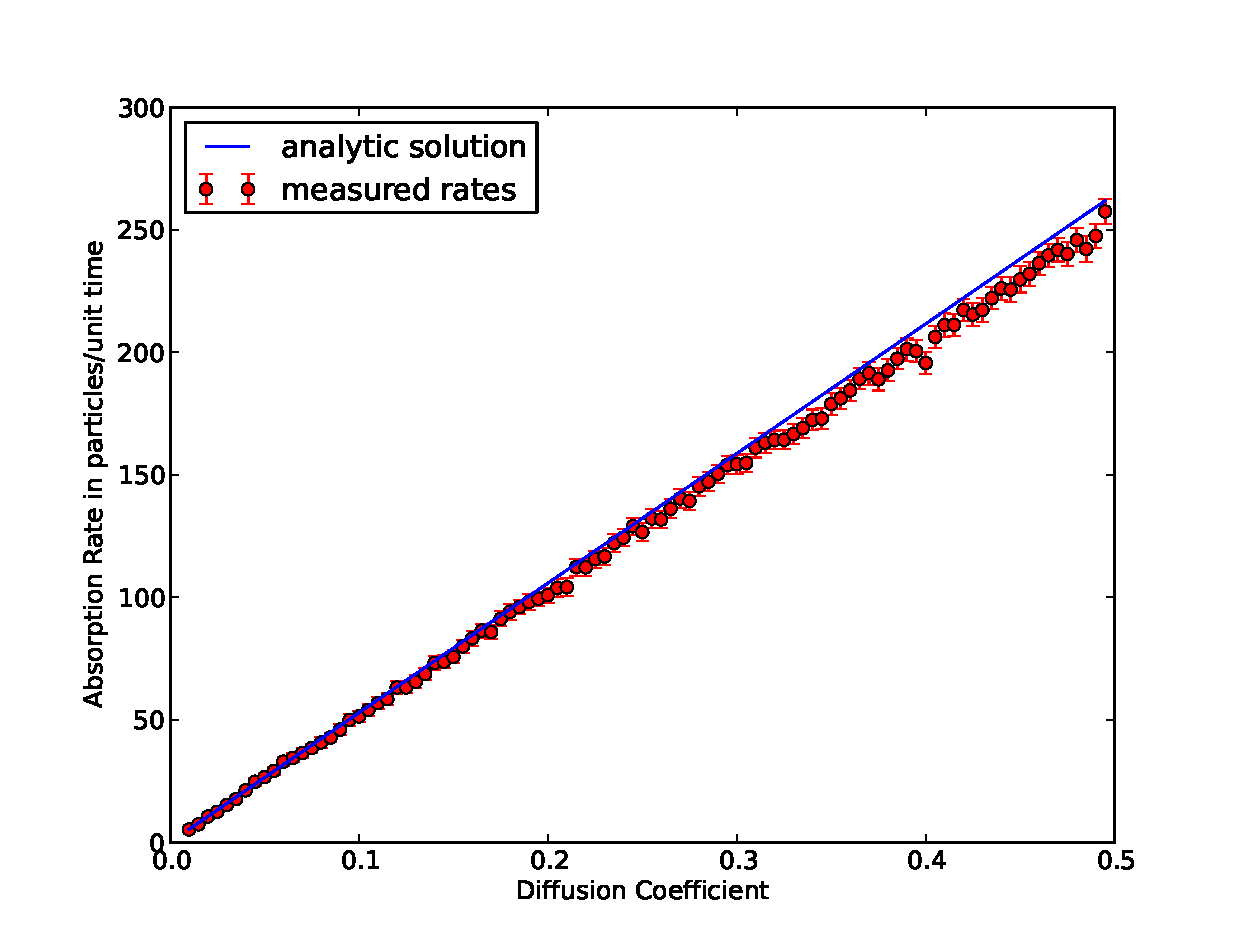
\includegraphics[width=.85 \textwidth, keepaspectratio]{plots/np/d/Kabs.eps}
    \caption{Reaction rates vs. Diffusion coefficient - Analytic solution and measured results}
    \label{fig:Kabs_D}
\end{figure}
\begin{wrapfigure}[17]{O}{.6 \textwidth}
    \centering
    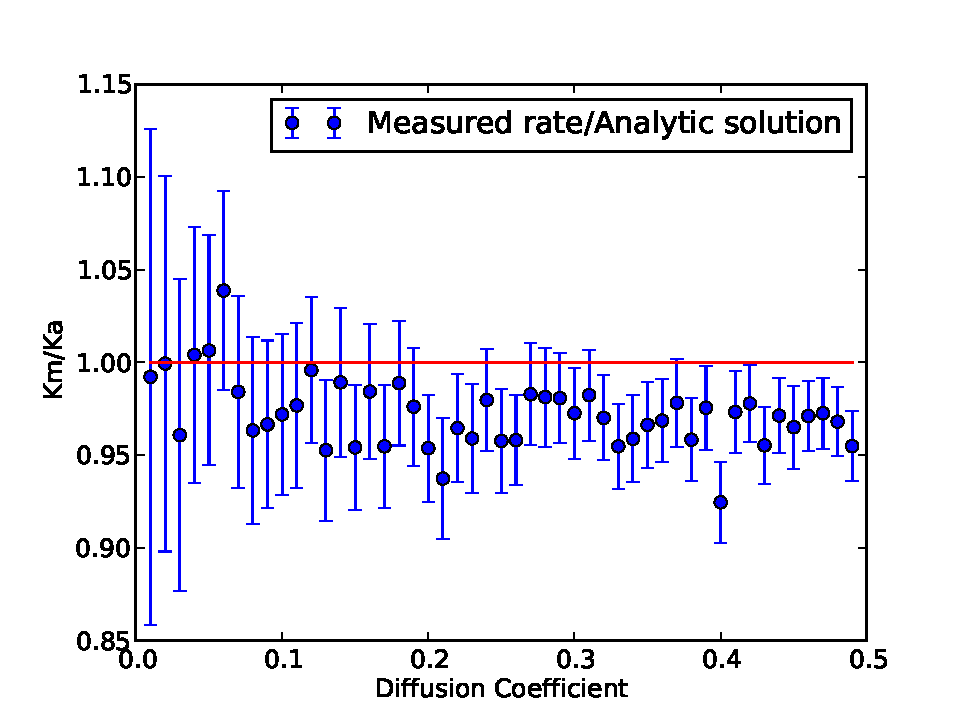
\includegraphics[width = .56 \textwidth, keepaspectratio]{plots/np/d/Krel.eps}
    \caption{Relative quantities for Reaction rates}
    \label{fig:Krel_d}
\end{wrapfigure}
The preceding figure shows the results for several simulation runs with different diffusion coefficient. It is obvious that the simulation results show the correct linear behaviour for the reaction rate but have a systematic error of about $5 - 10 \%$. To give a better impression of the relational dependence the following plot shows relative quantities for the results:
or $D > 0.1$ the figure shows a systematic error of about $5 \%$ in the results for the reaction rates. For $D<0.1$ the results are distributed around the analytic solution, mostly within the error bars, that are at  $2\sigma$. 
\newpage
\subsubsection{Varying Sink Radius $R_s$}
\begin{figure}[h]
    \centering
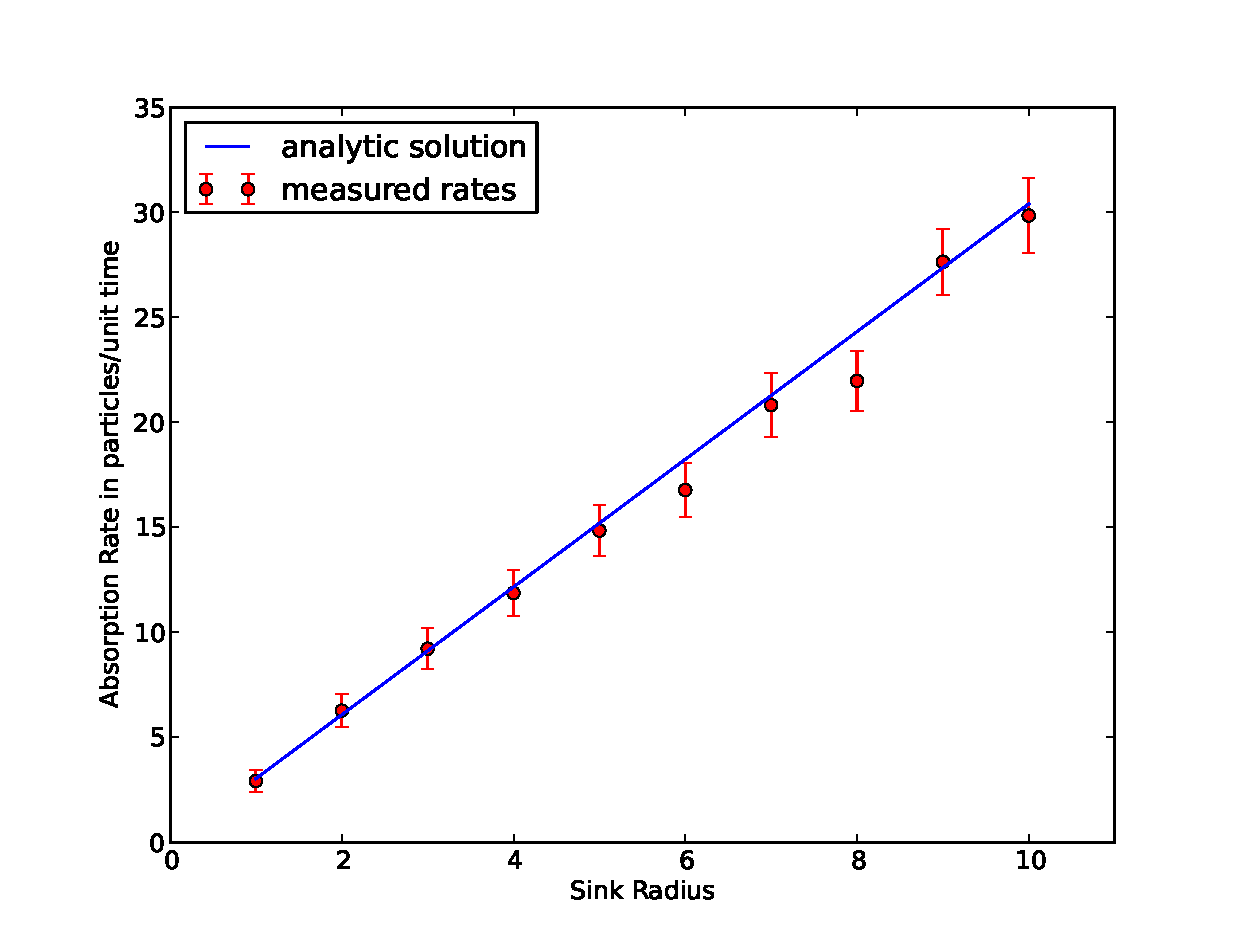
\includegraphics[width = .8 \textwidth]{plots/np/rs/KabsRs.eps}
    \caption{Reaction rate vs. Sink Radius}
    \label{fig:KabsRs}
\end{figure}
\begin{wrapfigure}[15]{O}{.6 \textwidth}
    \centering
    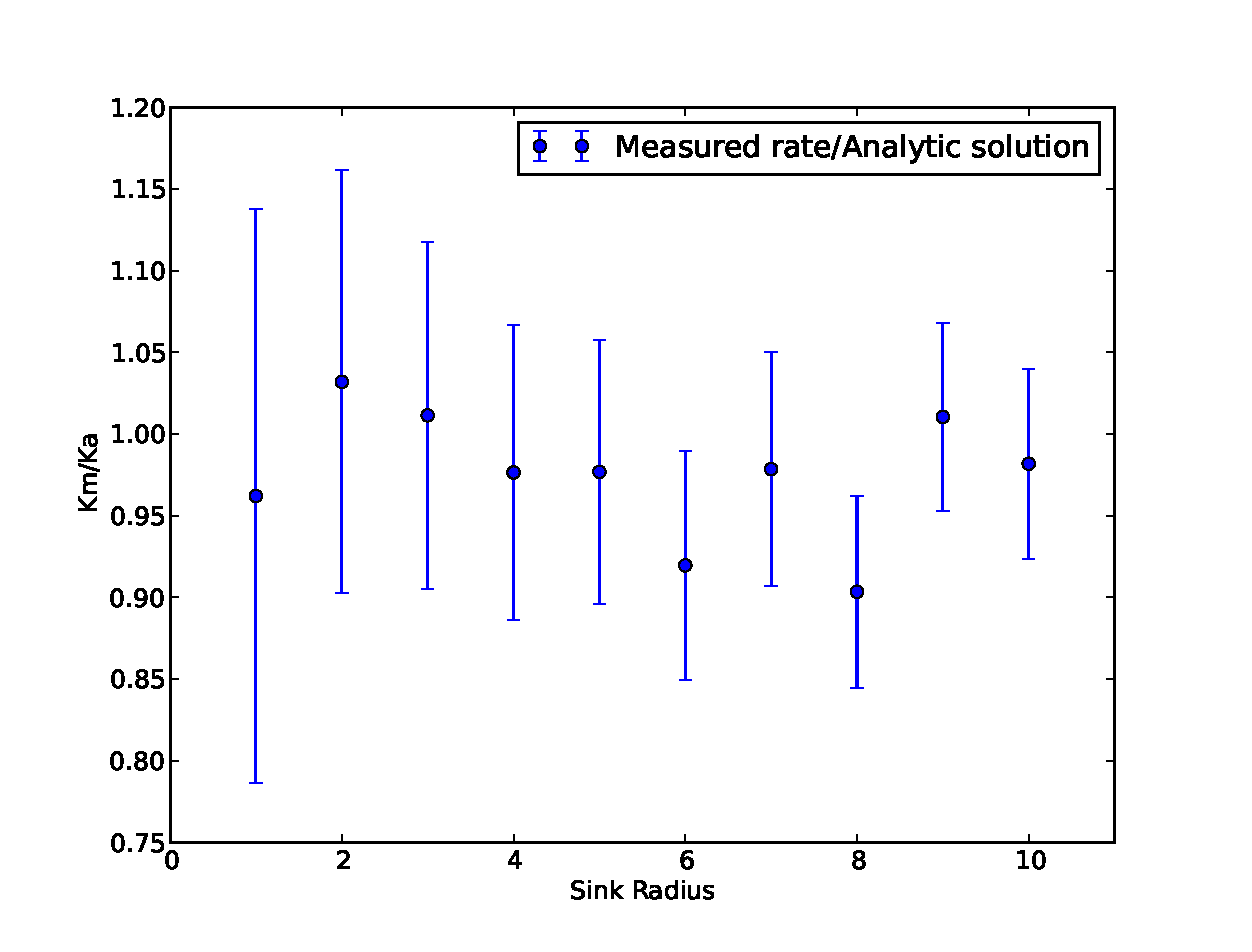
\includegraphics[width = .58 \textwidth]{plots/np/rs/KrelRs.eps}
    \caption{Normalized reaction rate vs. sink radius}
    \label{fig:KrelRs}
\end{wrapfigure}
This section gives results for different sink radius $R_s$ @ constant density $\rho_o$ to test the obvious linear relationship given in \eqref{Steady_state_rate}.
\
The results presented in the figure above do qualitatively support the linear relation between sink radius and reaction rate.
The adjacent strongly suggests, that the simulation also quantitatively maps on the analytic solution as the results are correct within the calculated errors at $2 \sigma$.
The following figures present the obtained density profiles from the simulation.
\begin{figure}[H]
    \centering
    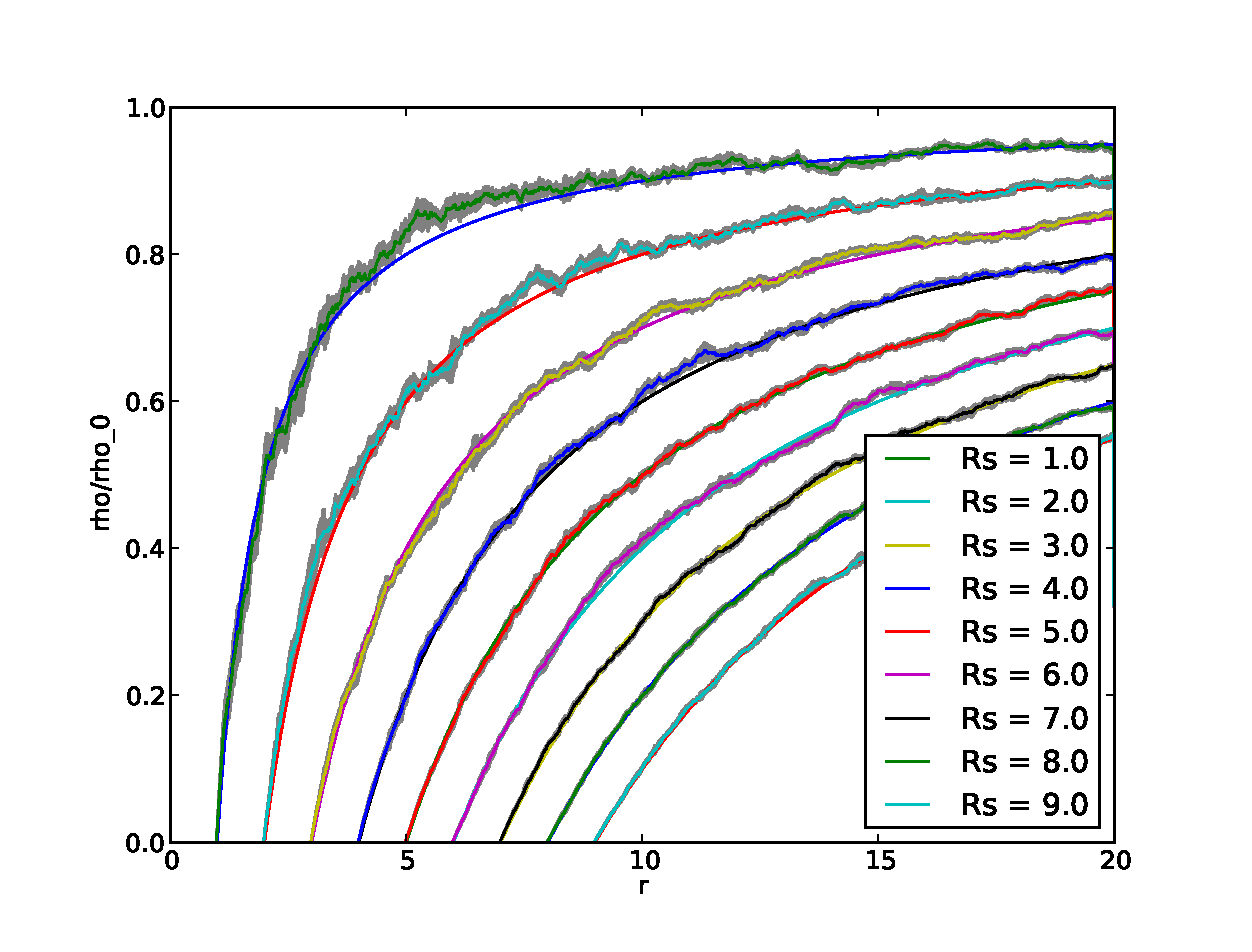
\includegraphics[width = .8 \textwidth]{plots/np/rs/rho_over_rho0.eps} 
    \caption{Normalized density profiles for different sink radius}
    \label{fig:ror0Rs}
\end{figure}
\begin{figure}[H]
    \centering
    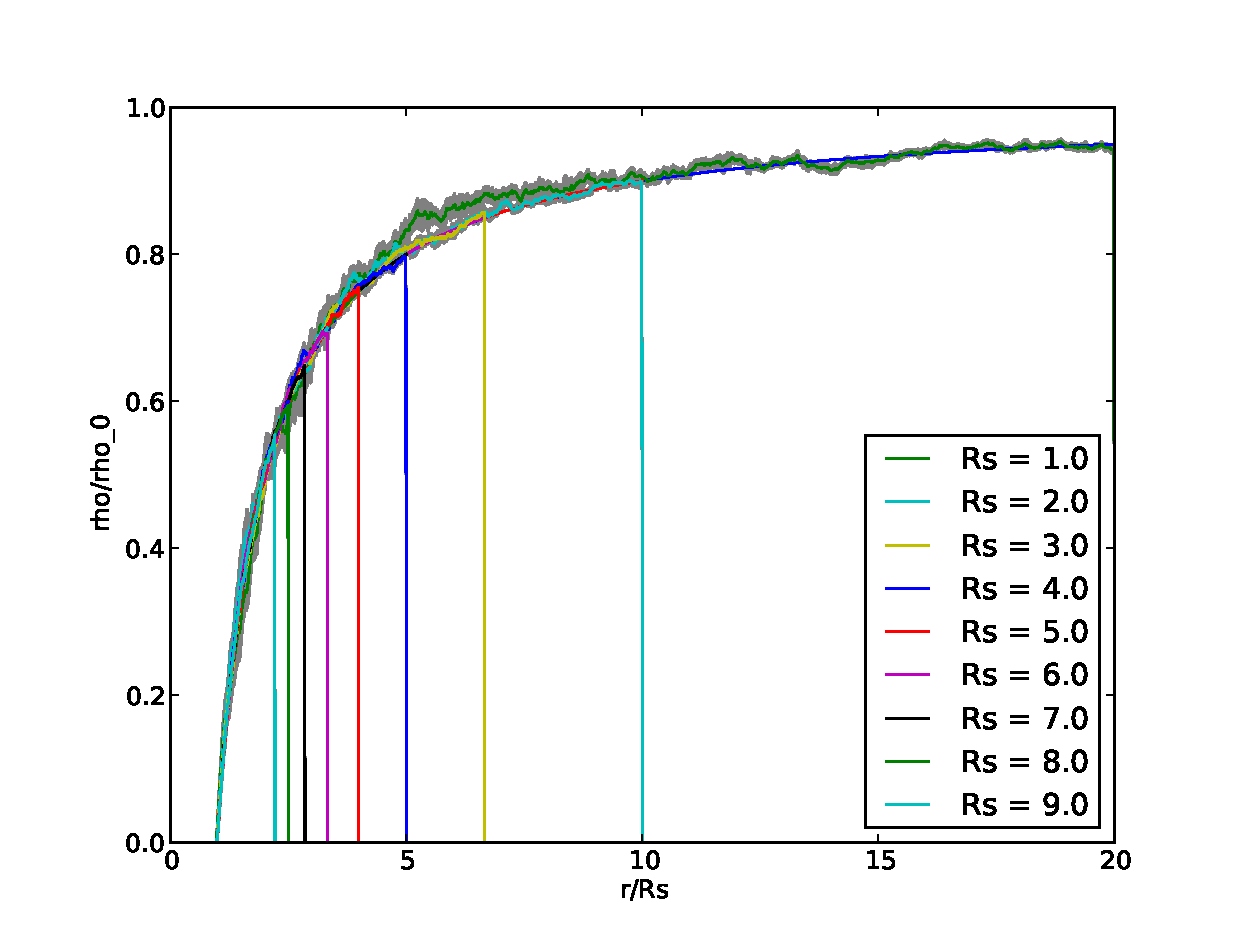
\includegraphics[width = .8 \textwidth]{plots/np/rs/rho_over_rho_0_rescaled.eps} 
    \caption{Normalized density profiles for different sink radius with rescaled radial coordinate}
    \label{fig:ror0Rs_rescaled}
\end{figure}
\newpage
\subsubsection{Finite size analysis - Varying Domain Radius $R_d$}
\begin{figure}[H]
    \centering
    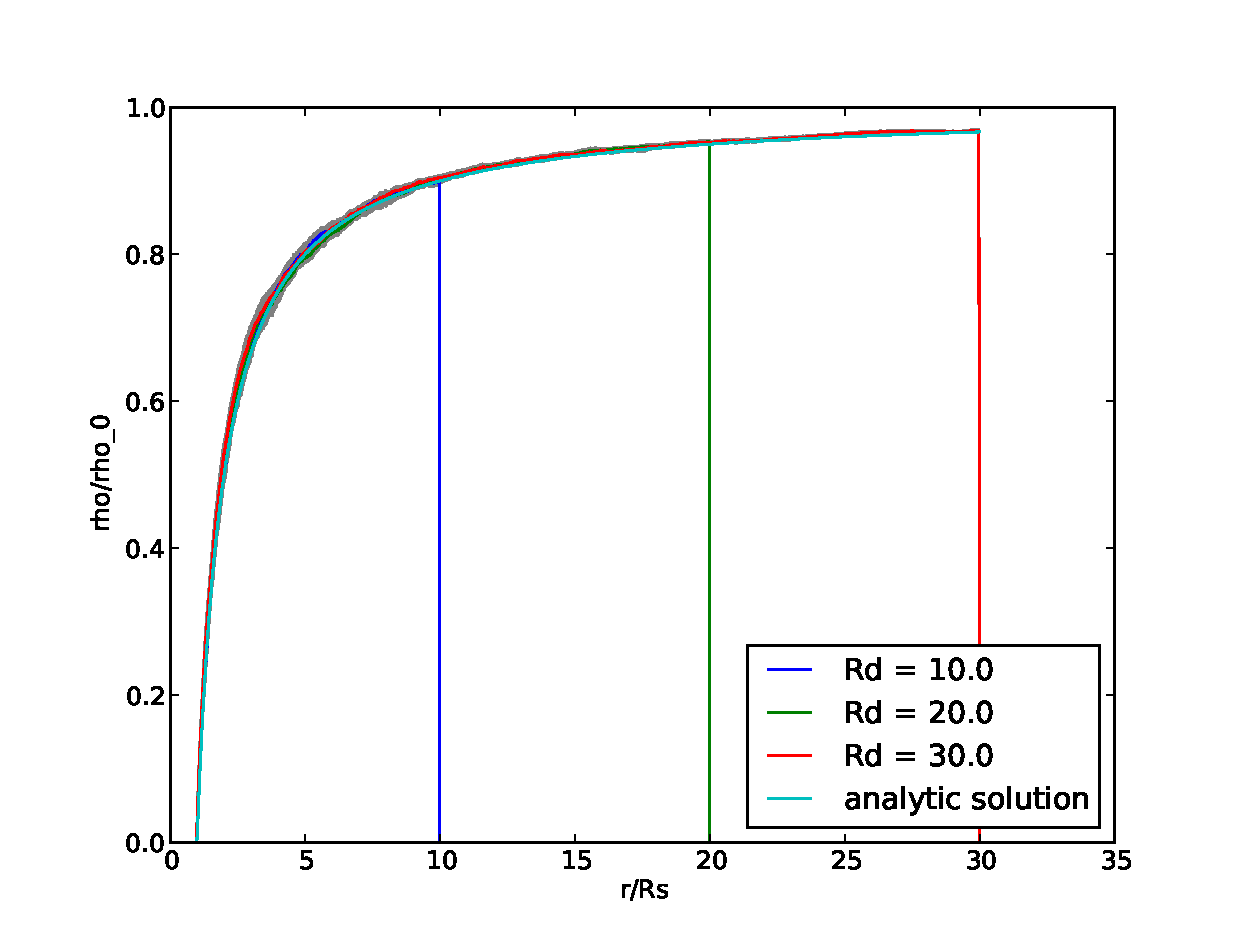
\includegraphics[width = .8 \textwidth]{plots/np/rd/rho_over_rho0.eps}
    \caption{Density profiles for different domain Radius $R_d$}
    \label{fig:ror0Rd}
\end{figure}
\begin{wrapfigure}[17]{O}{.6 \textwidth}
    \centering
    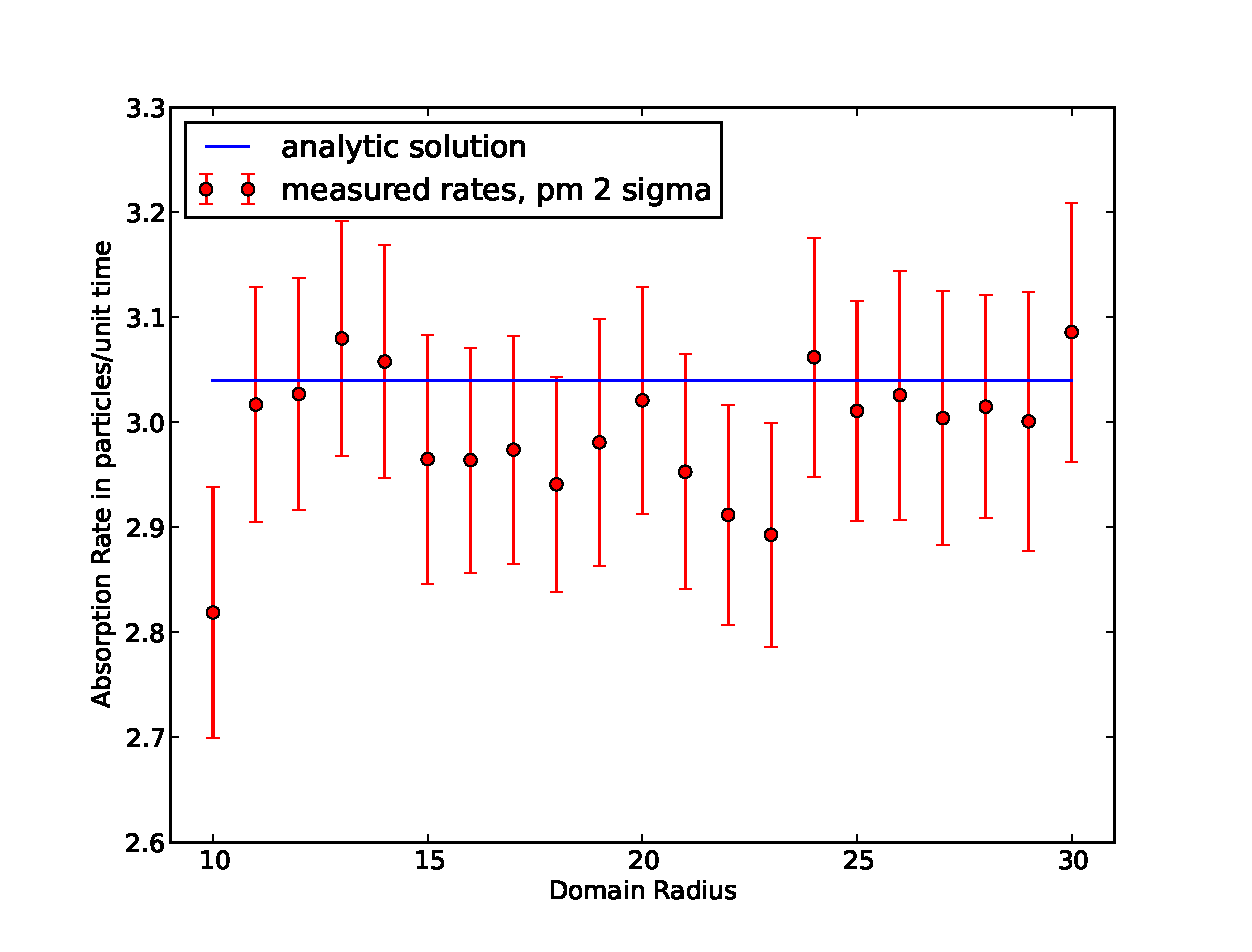
\includegraphics[width = .56 \textwidth]{plots/np/rd/KabsRd.eps}
    \caption{reaction rate vs. domain radius}
    \label{fig:KrelRd}
\end{wrapfigure}
This section shows plots for different domain radius $R_d$ @ constant density $\rho_o$.
This will point out finite size effects in the simulation (if they exist). To account for the larger volume the number of particles is adjusted to keep the solution for density profile and rate constants unchanged.
The plot above shows, that the variation of the domain radius does not qualitatively change the simulated density profile. \\
The results for the rate constants does not show any qualitative changes for varying domain radius. \\
These results suggest, that for the given boundary conditions and for ideal particles without external forces there are no finite size effects in this simulation.
\subsection{Subsumption}
The different results from simulation presented in the previous section show that:
\begin{itemize}
    \item The density profiles from the BD simulation fit the analytical solution,
    \item the obtained rate constants are as expected within the calculated errors
    \item   the diffusion constant and  or time step has to be small enough for the particle 
            trajectories to resolve the boundary conditions properly,
    \item finite size effects can be neglected.
\end{itemize}
\subsection{Ideal Sink with Boxcar Potential Barrier}
The following section contains simulation results for a potential barrier as derived in \eqref{Boxcar_solution}. If not stated differently, the following parameters are used:
\begin{table}[H]
    \centering
    \begin{tabular}{r|l}
        $N$ & $10^{4}$\\
        $D$ & $0,05$\\
        $R_s$ & $1$ \\
        $R_d$ & $10$ \\
        $U_0$ & $2$ \\
        $U_a$ & $2$ \\
        $U_b$ & $2$ \\
        $U_n$ & $50$ \\
        ${\rm d}t$ & $10^{-4}$
    \end{tabular}
    \caption{Default simulation parameters for simulation with boxcar potential}
    \label{tab:Parameters_cp}
\end{table}

\subsubsection{Varying Distance from Sink to Barrier ($U_a$)}
\begin{figure}[H]
\centering
\begin{minipage}{.5 \textwidth}
    \centering
    \includegraphics[width=.95 \textwidth, keepaspectratio]{plots/cp/ua/Ua1.eps}
\end{minipage}\begin{minipage}{.5 \textwidth}
    \includegraphics[width=.95 \textwidth, keepaspectratio]{plots/cp/ua/Ua3.eps}
\end{minipage}
\begin{minipage}{.5 \textwidth}
    \includegraphics[width=.95 \textwidth, keepaspectratio]{plots/cp/ua/Ua5.eps}
\end{minipage}\begin{minipage}{.5 \textwidth}
    \includegraphics[width=.95 \textwidth, keepaspectratio]{plots/cp/ua/Ua5.eps}
\end{minipage}
 
    \caption{Density Profile for varying $U_a$}
    \label{fig:RhoUaCp}
\end{figure}

The simulation results obviously fit the analytic solution. Same holds for the calculated reaction rates as presented in the following Plot:
\begin{figure}[H]
\centering
\begin{minipage}{.5 \textwidth}
    \centering
    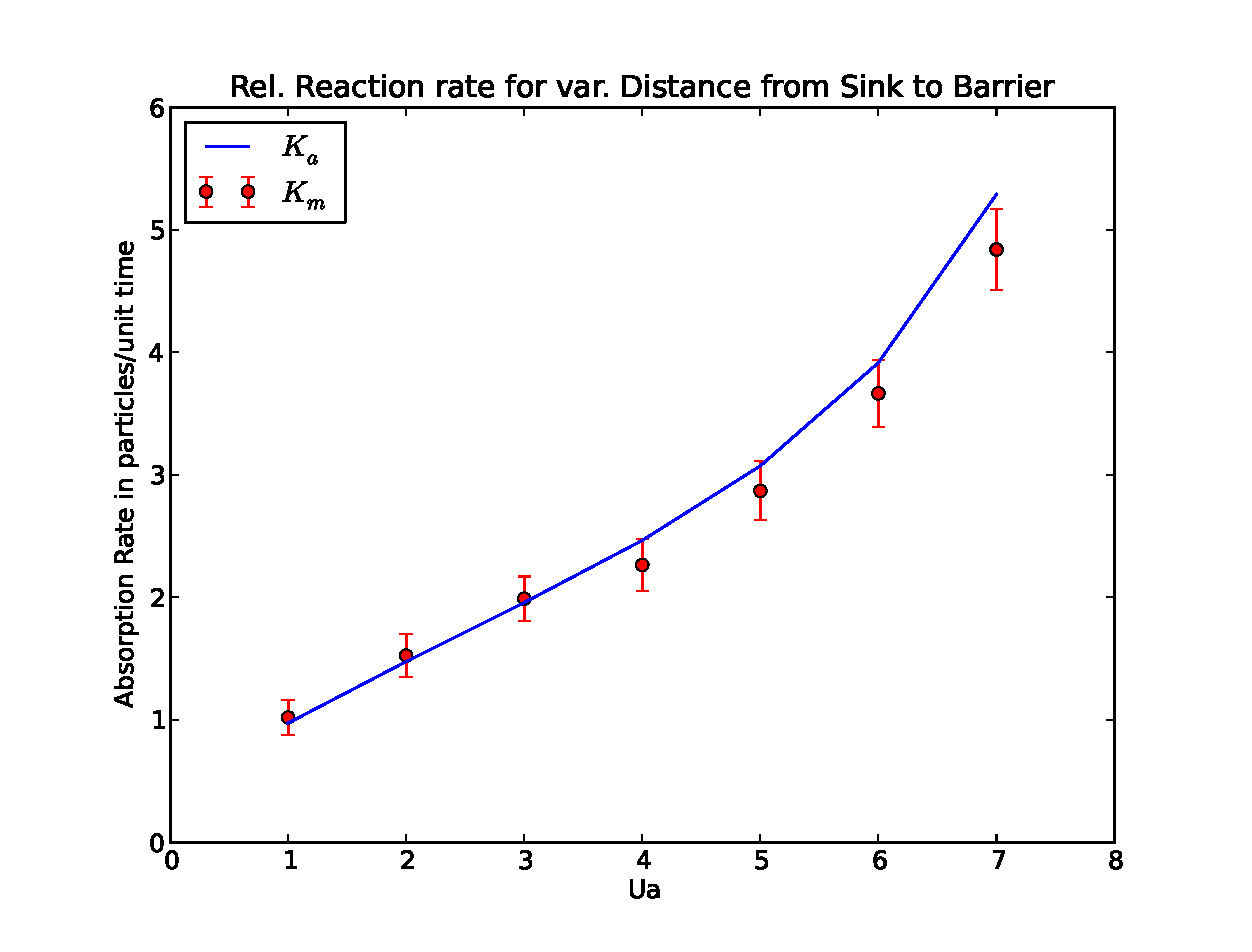
\includegraphics[width=.95 \textwidth, keepaspectratio]{plots/cp/ua/Kabs.eps}
\end{minipage}\begin{minipage}{.5 \textwidth}
    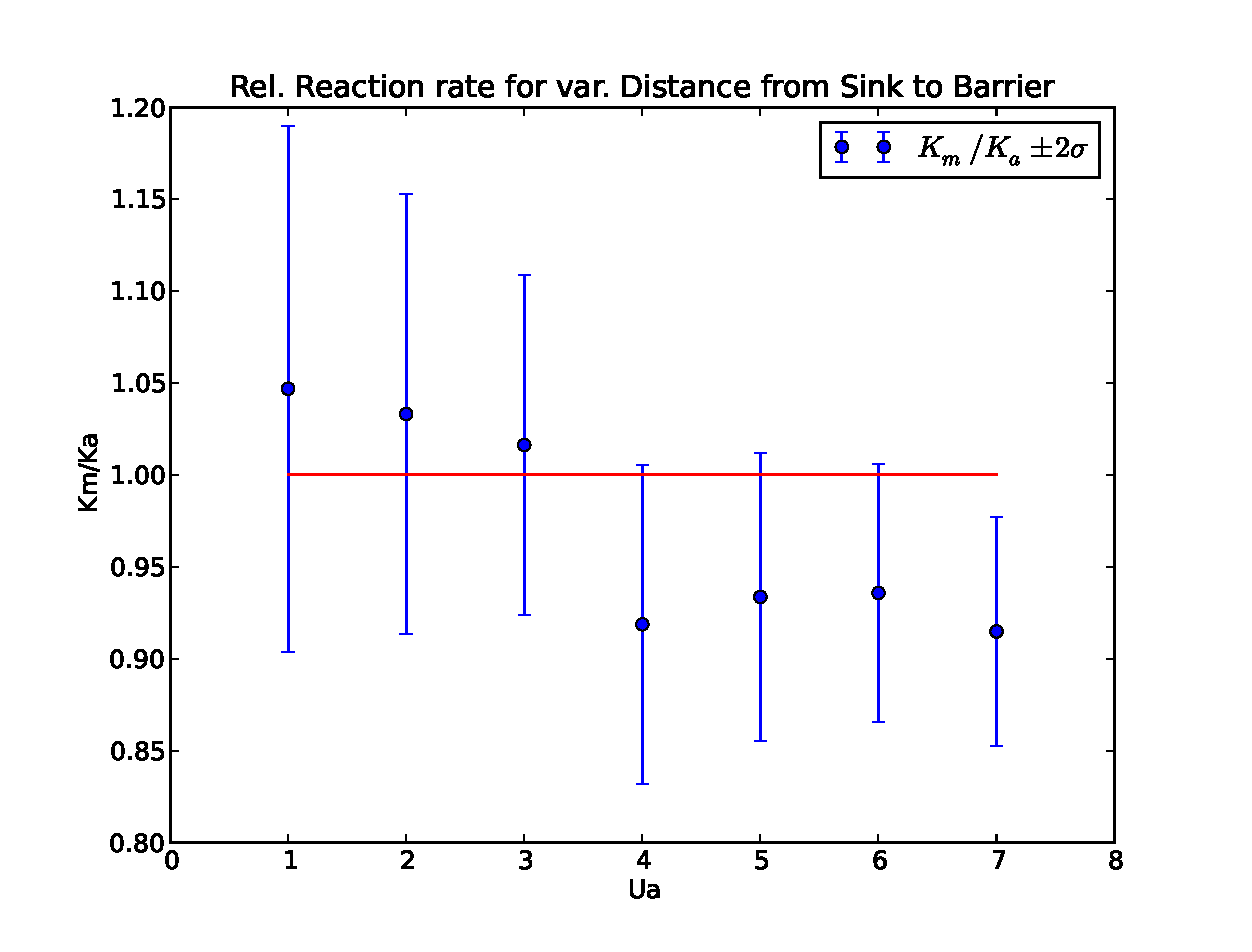
\includegraphics[width=.95 \textwidth, keepaspectratio]{plots/cp/ua/Krel.eps}
\end{minipage}
\caption{Absolute and relative Absorption rate for varying $U_a$}
\label{fig:KUaCp}
\end{figure}

\subsubsection{Varying Barrier Height ($U_0$)}
\begin{figure}[H]
\centering
\begin{minipage}{.5 \textwidth}
    \centering
    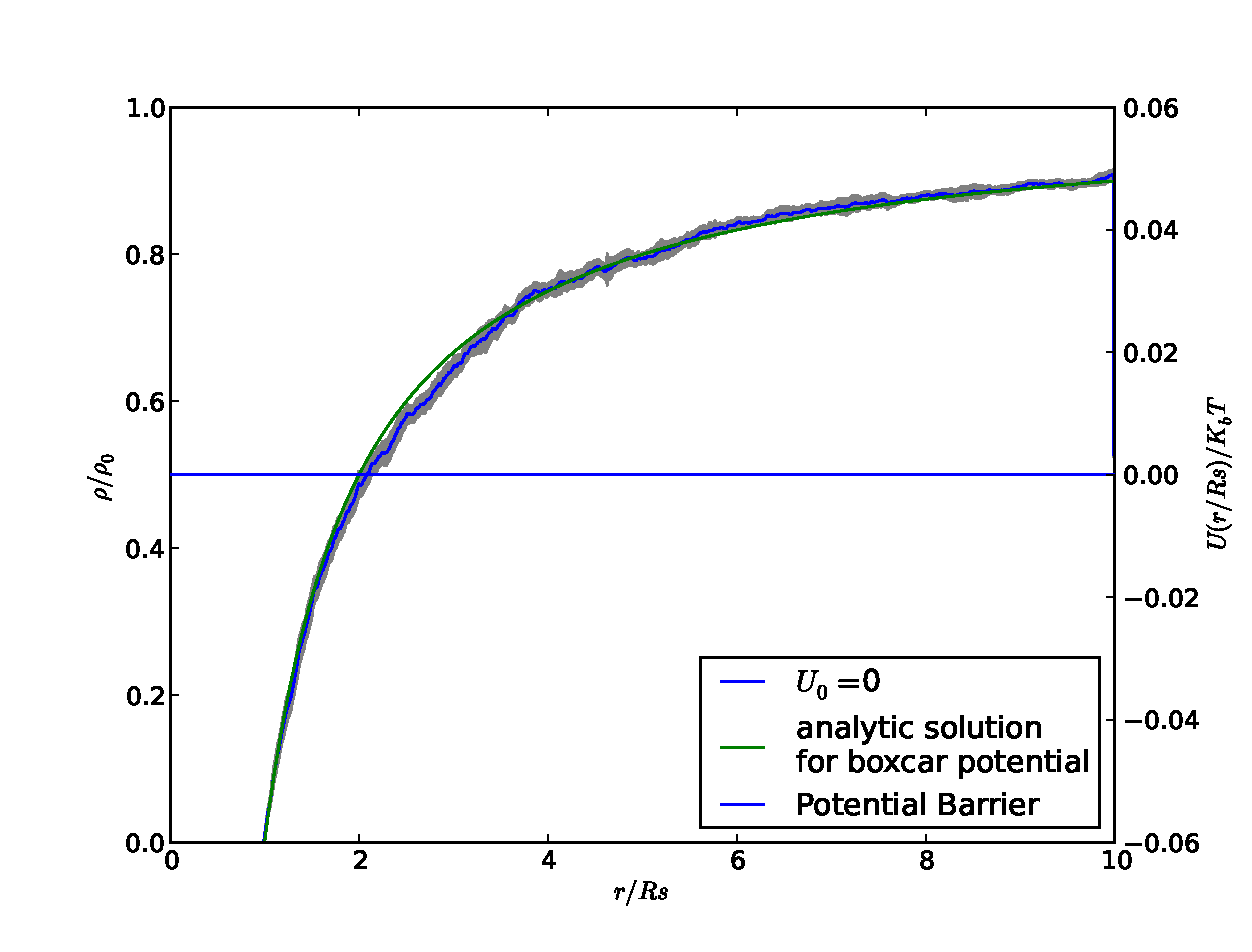
\includegraphics[width=.95 \textwidth, keepaspectratio]{plots/cp/uo/Un0.eps}
\end{minipage}\begin{minipage}{.5 \textwidth}
    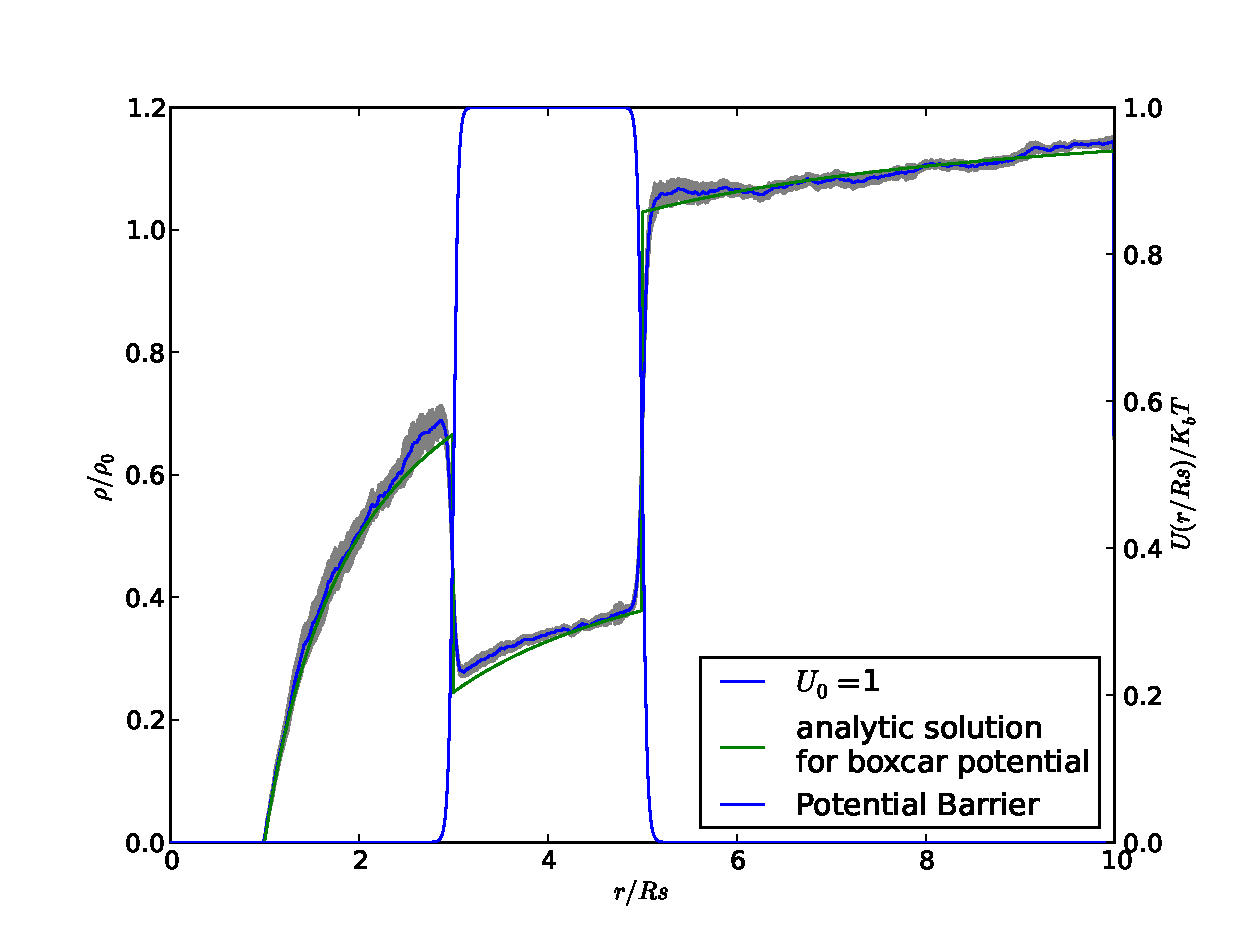
\includegraphics[width=.95 \textwidth, keepaspectratio]{plots/cp/uo/Un1.eps}
\end{minipage}
\begin{minipage}{.5 \textwidth}
    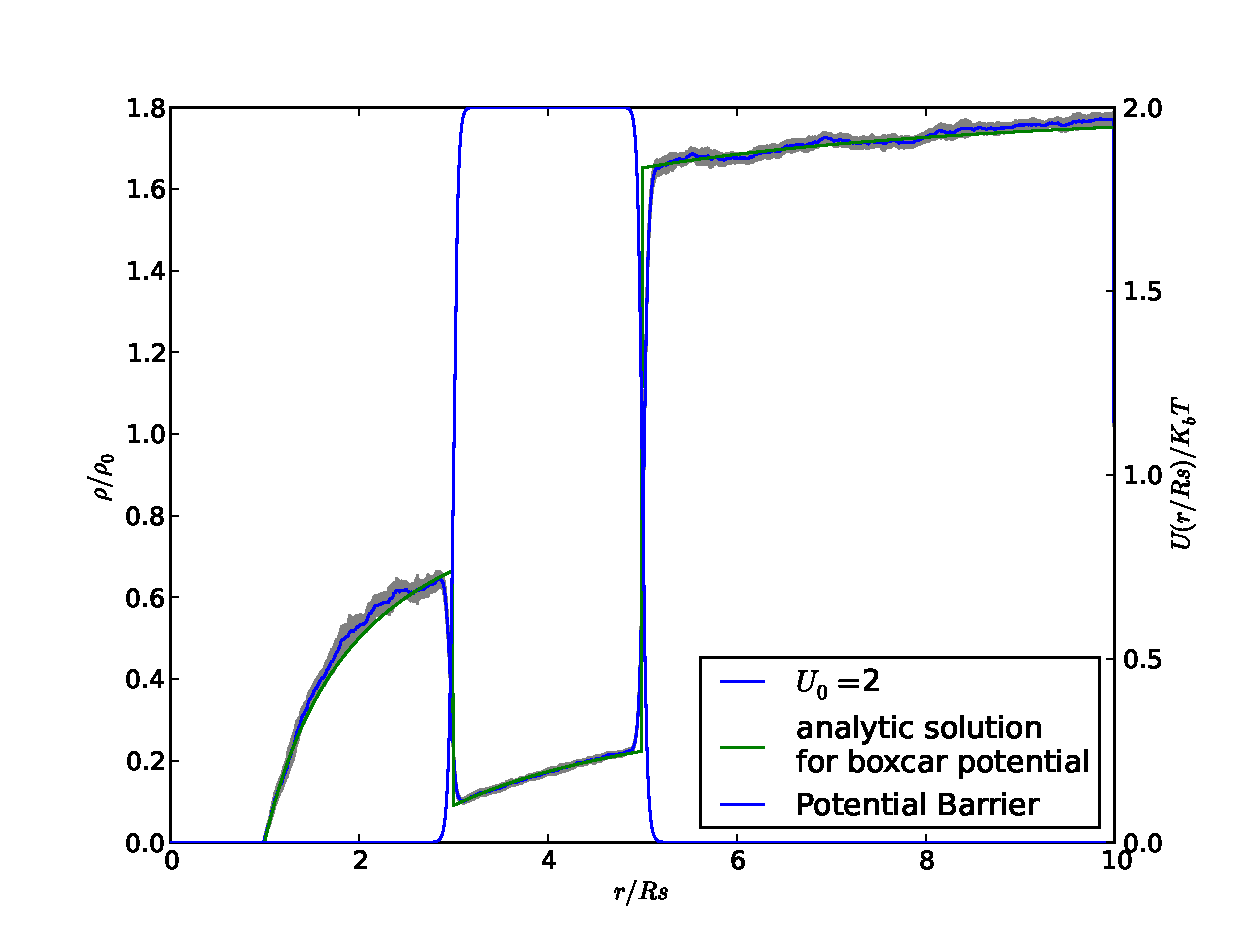
\includegraphics[width=.95 \textwidth, keepaspectratio]{plots/cp/uo/Un2.eps}
\end{minipage}\begin{minipage}{.5 \textwidth}
    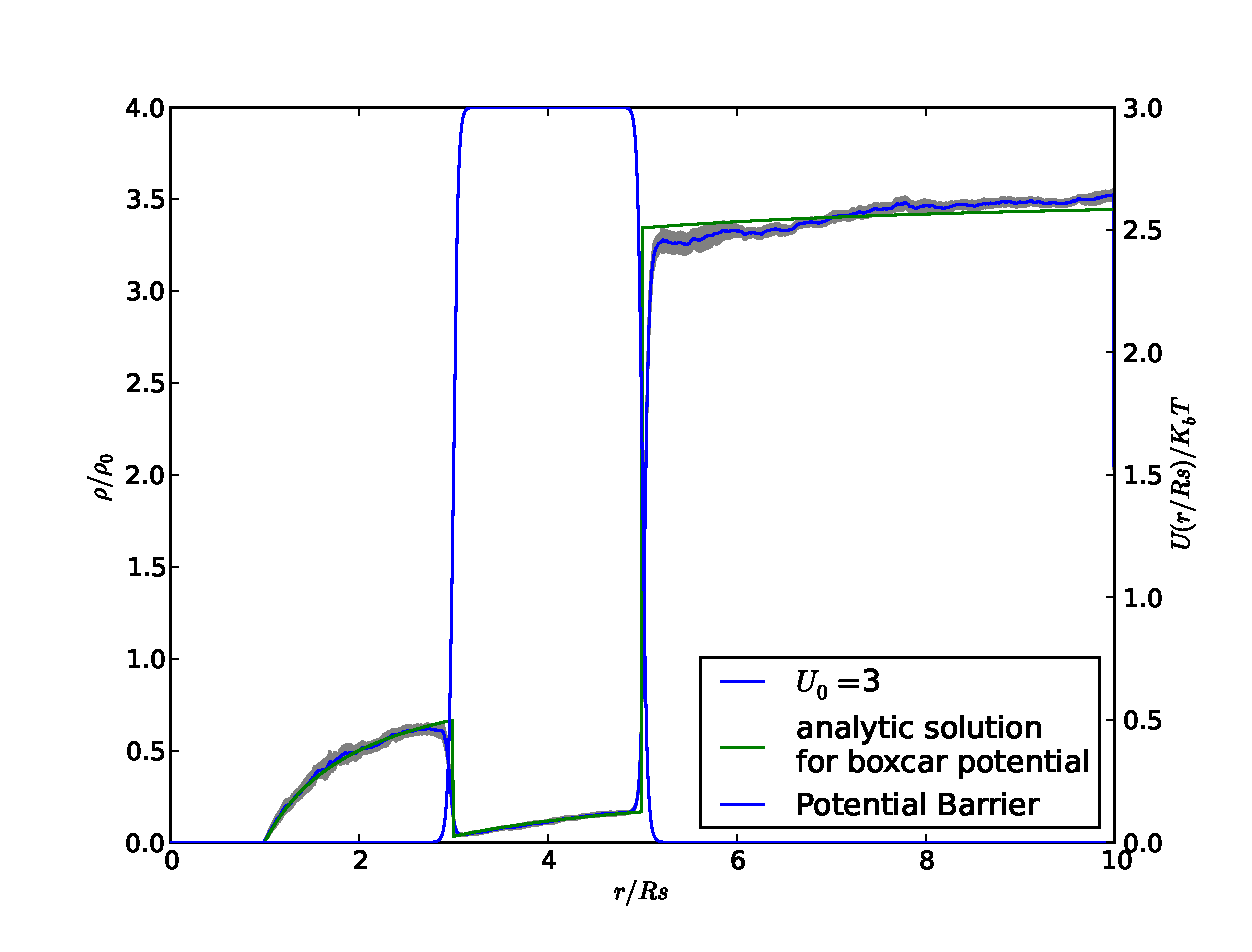
\includegraphics[width=.95 \textwidth, keepaspectratio]{plots/cp/uo/Un3.eps}
\end{minipage}
 
    \caption{Density Profile for varying $U_0$}
    \label{fig:RhoU0Cp}
\end{figure}

The simulation results obviously fit the analytic solution. Same holds for the calculated reaction rates as presented in the following Plot:
\begin{figure}[H]
\centering
\begin{minipage}{.5 \textwidth}
    \centering
    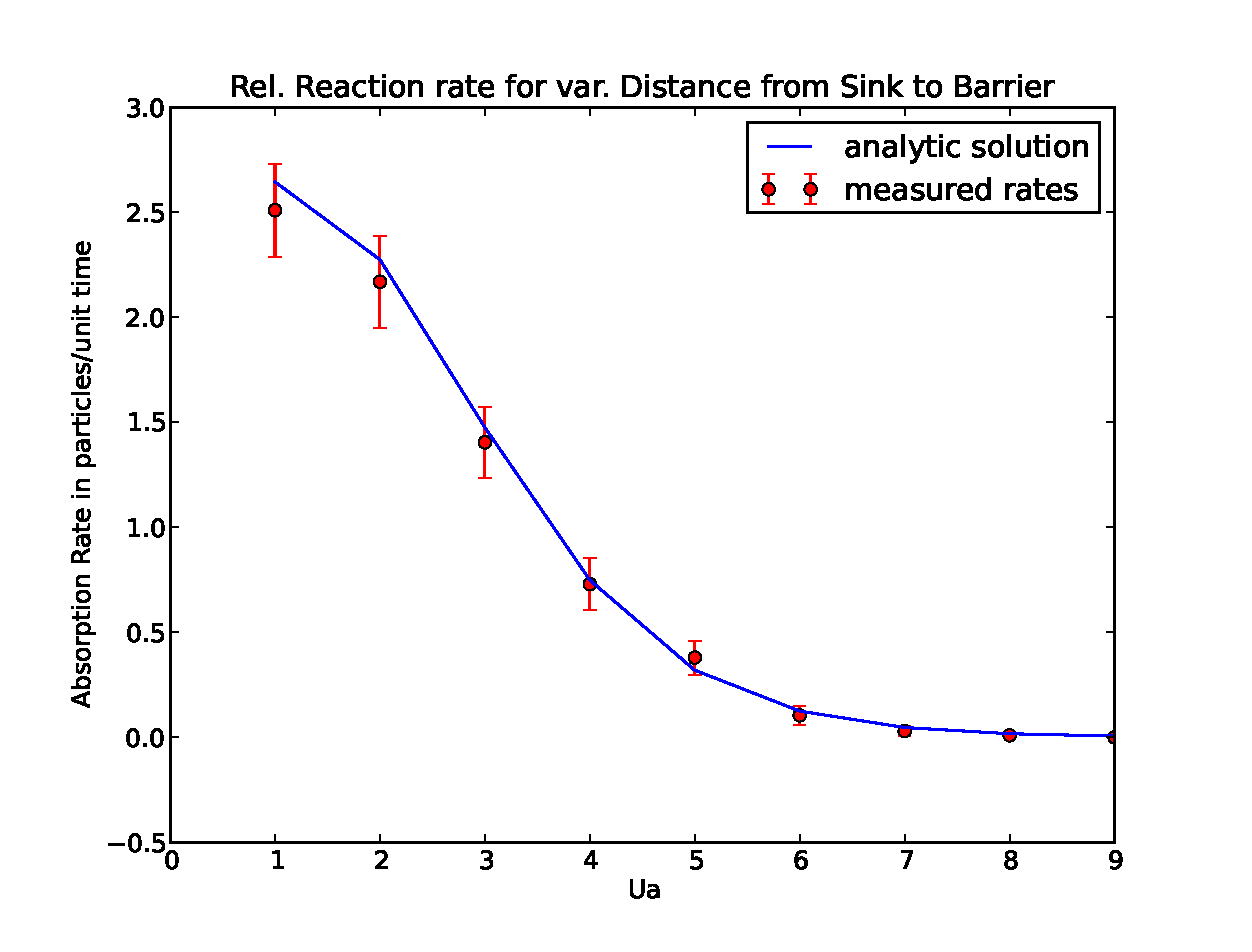
\includegraphics[width=.95 \textwidth, keepaspectratio]{plots/cp/uo/Kabs.eps}
\end{minipage}\begin{minipage}{.5 \textwidth}
    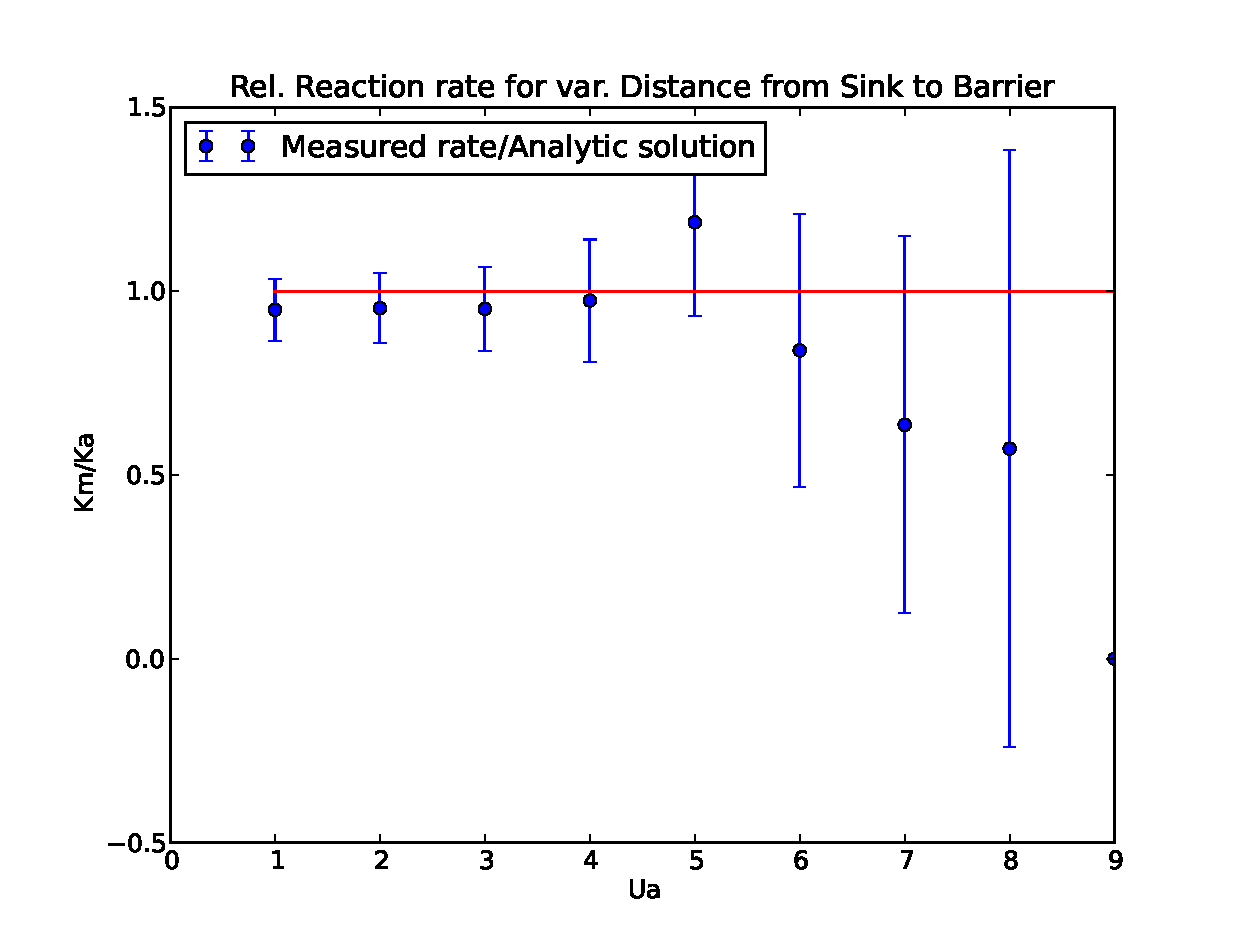
\includegraphics[width=.95 \textwidth, keepaspectratio]{plots/cp/uo/Krel.eps}
\end{minipage}
\caption{Absolute and relative Absorption rate for varying $U_0$}
\label{fig:KU0Cp}
\end{figure}


\subsubsection{Varying Barrier Steepness ($U_n$)}
\begin{figure}[H]
\centering
\begin{minipage}{.5 \textwidth}
    \centering
    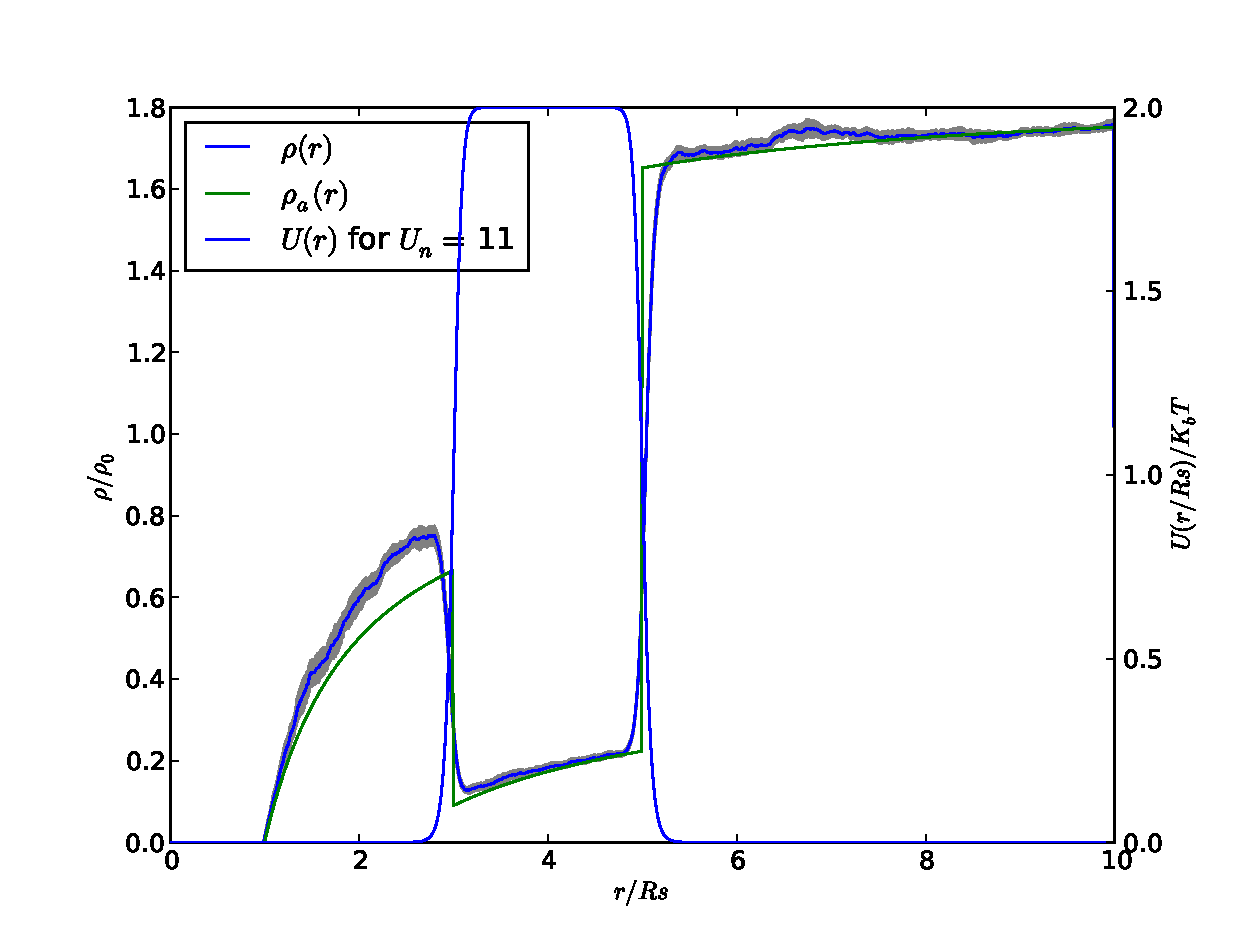
\includegraphics[width=.95 \textwidth, keepaspectratio]{plots/cp/un/Un11.eps}
\end{minipage}\begin{minipage}{.5 \textwidth}
    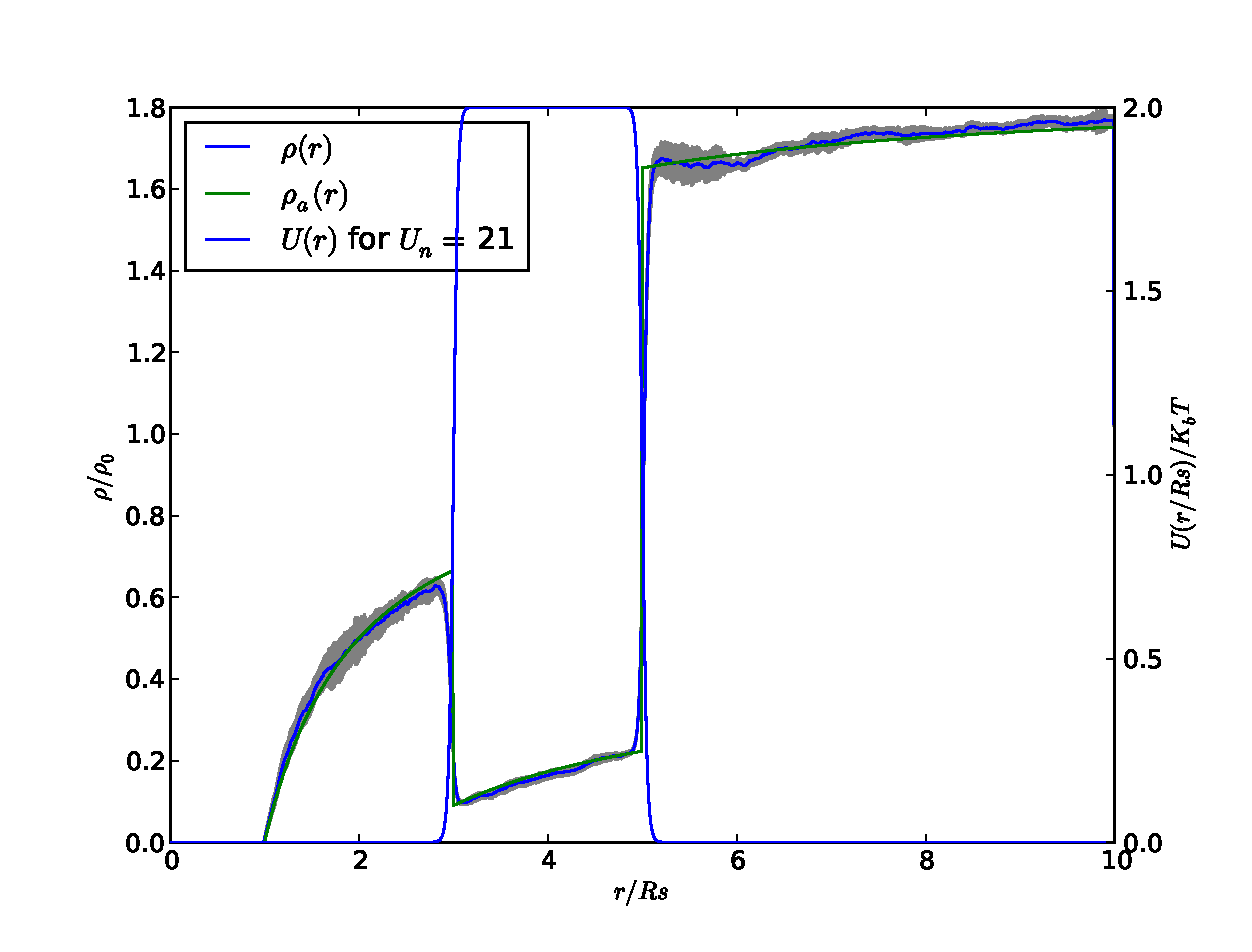
\includegraphics[width=.95 \textwidth, keepaspectratio]{plots/cp/un/Un21.eps}
\end{minipage}
\begin{minipage}{.5 \textwidth}
    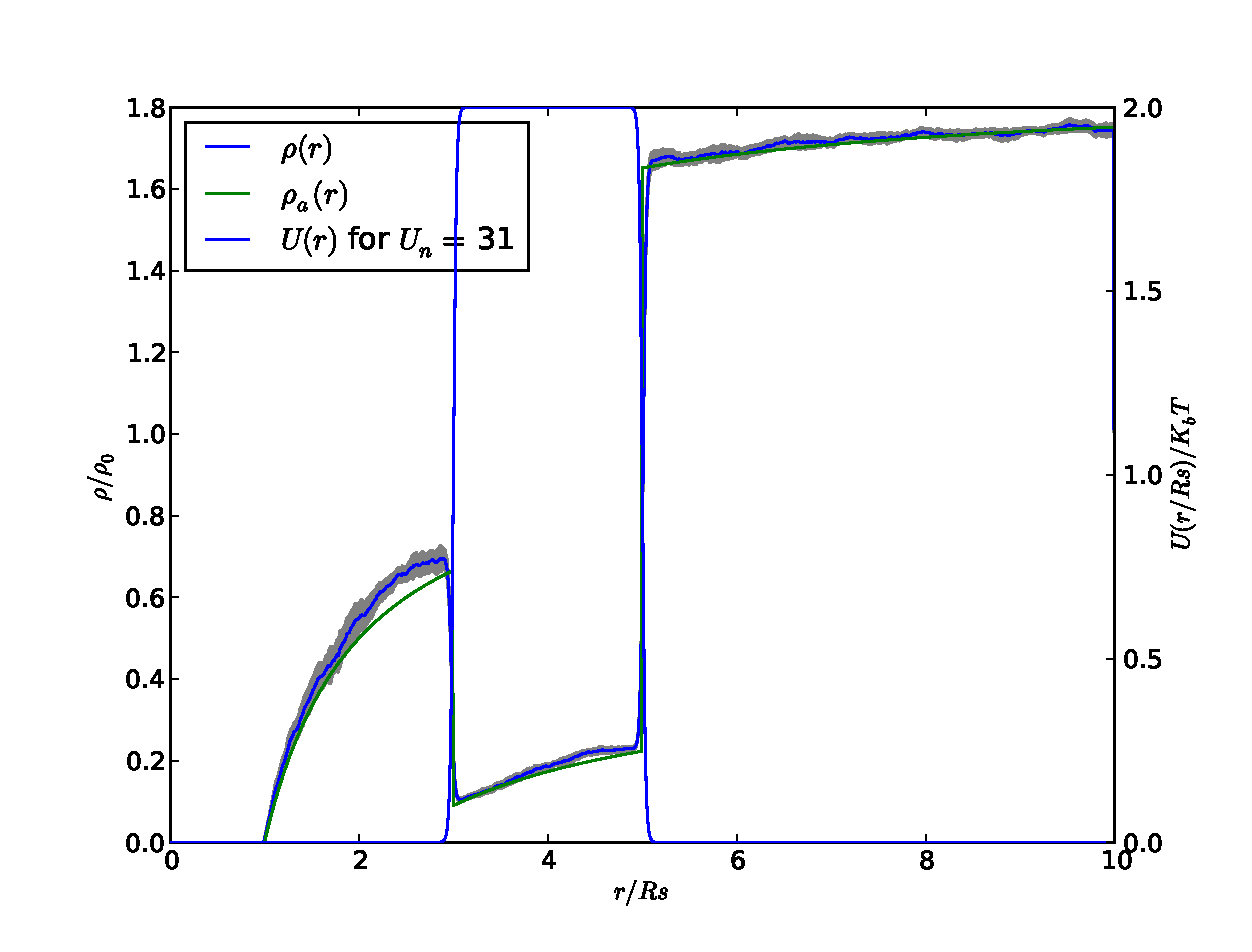
\includegraphics[width=.95 \textwidth, keepaspectratio]{plots/cp/un/Un31.eps}
\end{minipage}\begin{minipage}{.5 \textwidth}
    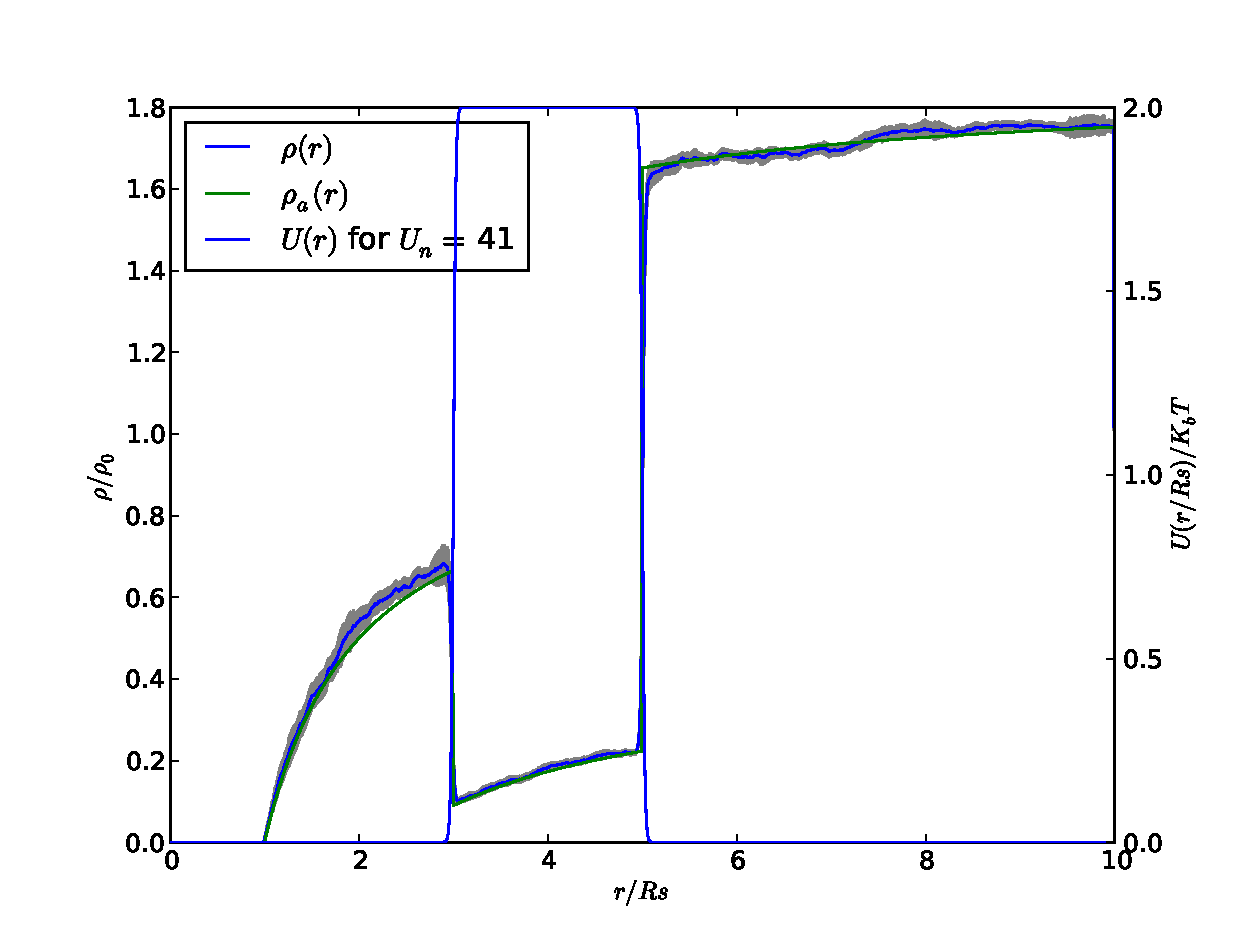
\includegraphics[width=.95 \textwidth, keepaspectratio]{plots/cp/un/Un41.eps}
\end{minipage}
 
    \caption{Density Profile for varying $U_n$}
    \label{fig:RhoUnCp}
\end{figure}

The simulation results obviously fit the analytic solution. Same holds for the calculated reaction rates as presented in the following Plot:
\begin{figure}[H]
\centering
\begin{minipage}{.5 \textwidth}
    \centering
    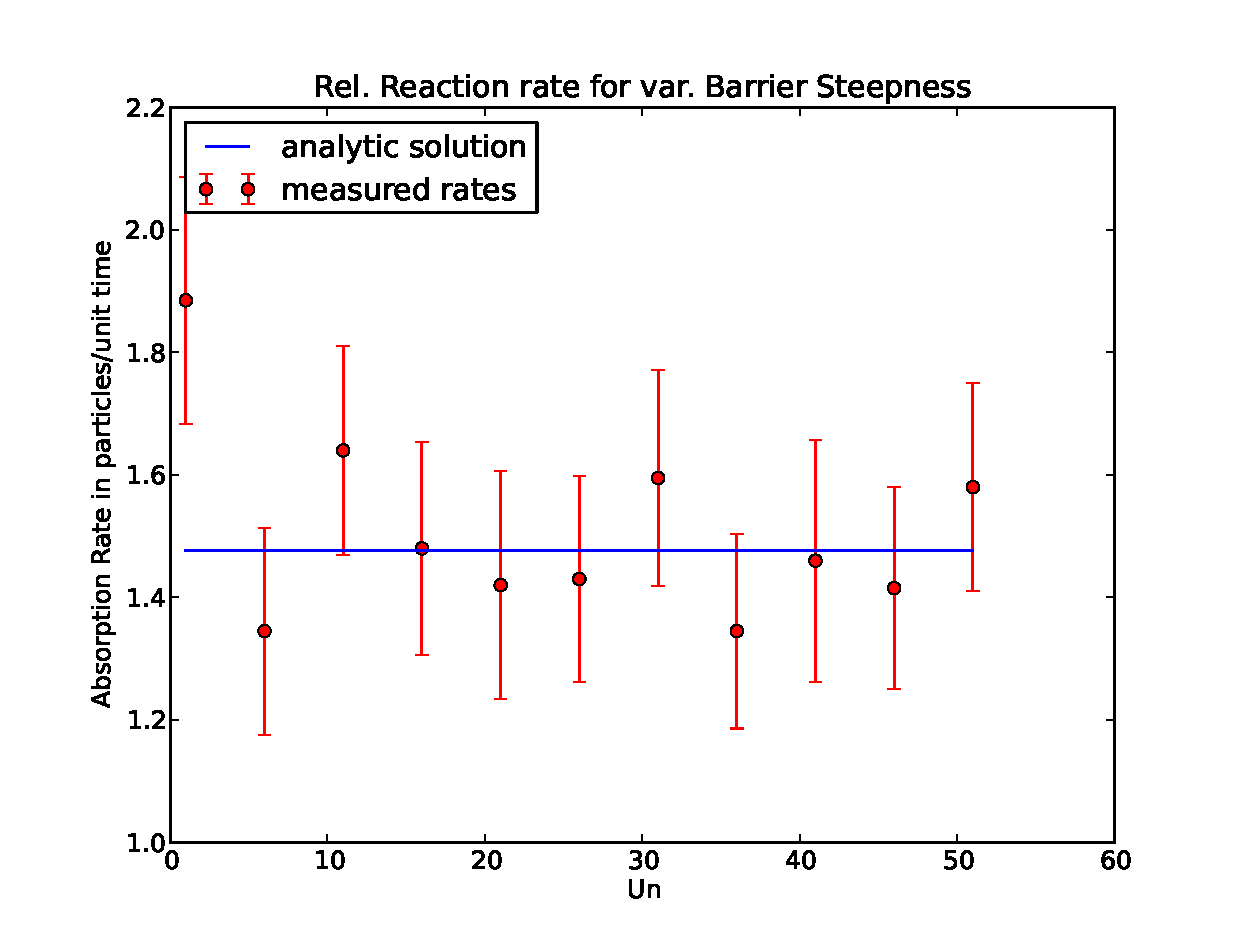
\includegraphics[width=.95 \textwidth, keepaspectratio]{plots/cp/un/Kabs.eps}
\end{minipage}\begin{minipage}{.5 \textwidth}
    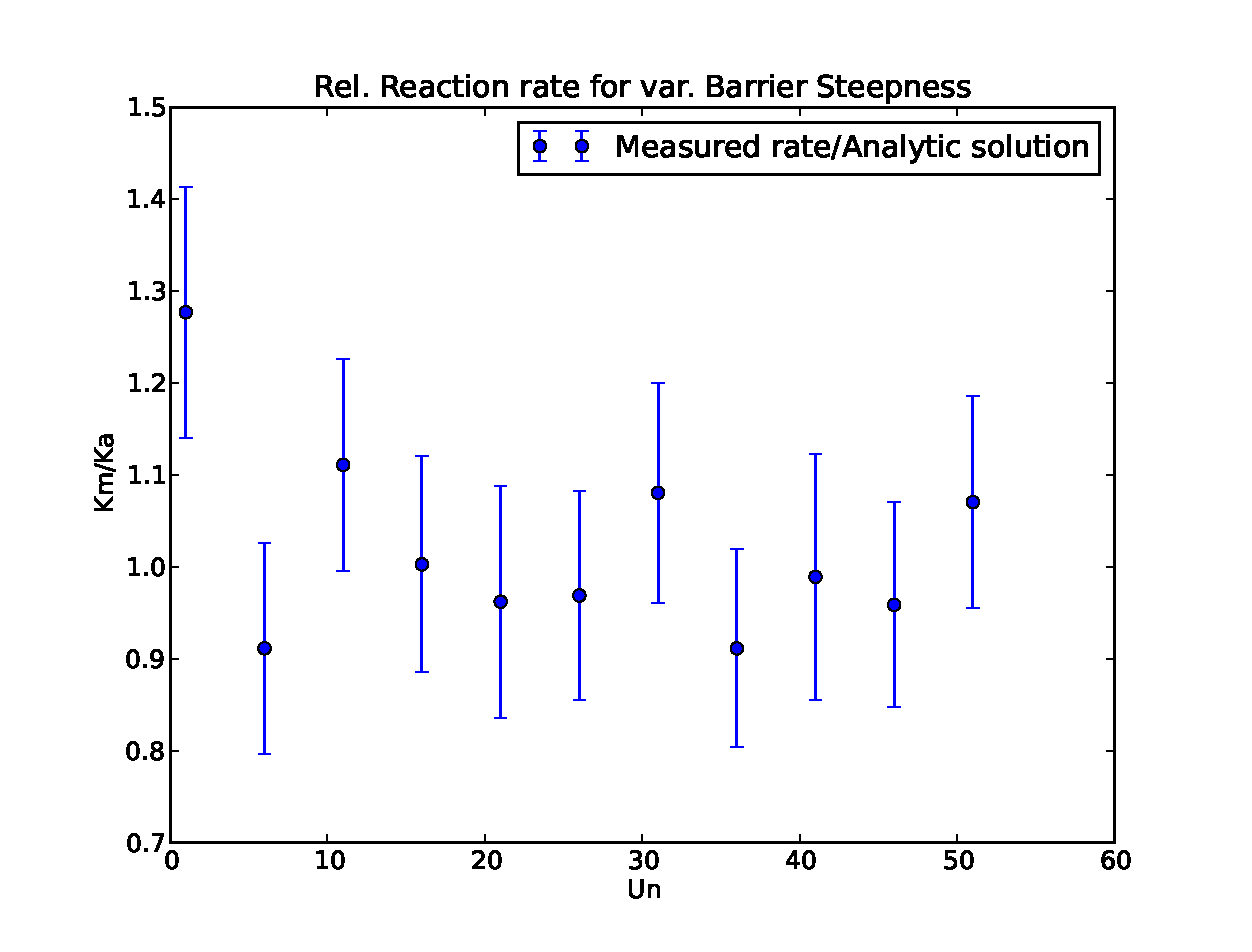
\includegraphics[width=.95 \textwidth, keepaspectratio]{plots/cp/un/Krel.eps}
\end{minipage}
\caption{Absolute and relative Absorption rate for varying $U_n$}
\label{fig:KUnCP}
\end{figure}


%\subsubsection{Varying Barrier Width}
%\begin{figure}[H]
%\centering
%\begin{minipage}{.5 \textwidth}
%    \centering
%    \includegraphics[width=.95 \textwidth, keepaspectratio]{plots/cp/ub/Ua1.eps}
%\end{minipage}\begin{minipage}{.5 \textwidth}
%    \includegraphics[width=.95 \textwidth, keepaspectratio]{plots/cp/ub/Ua3.eps}
%\end{minipage}
%\begin{minipage}{.5 \textwidth}
%    \includegraphics[width=.95 \textwidth, keepaspectratio]{plots/cp/ub/Ua5.eps}
%\end{minipage}\begin{minipage}{.5 \textwidth}
%    \includegraphics[width=.95 \textwidth, keepaspectratio]{plots/cp/ub/Ua5.eps}
%\end{minipage}
% 
%    \caption{Density Profile for varying $U_b$}
%    \label{fig:RhoUbCp}
%\end{figure}
%
%The simulation results obviously fit the analytic solution. Same holds for the calculated reaction rates as presented in the following Plot:
%\begin{figure}[H]
%\centering
%\begin{minipage}{.5 \textwidth}
%    \centering
%    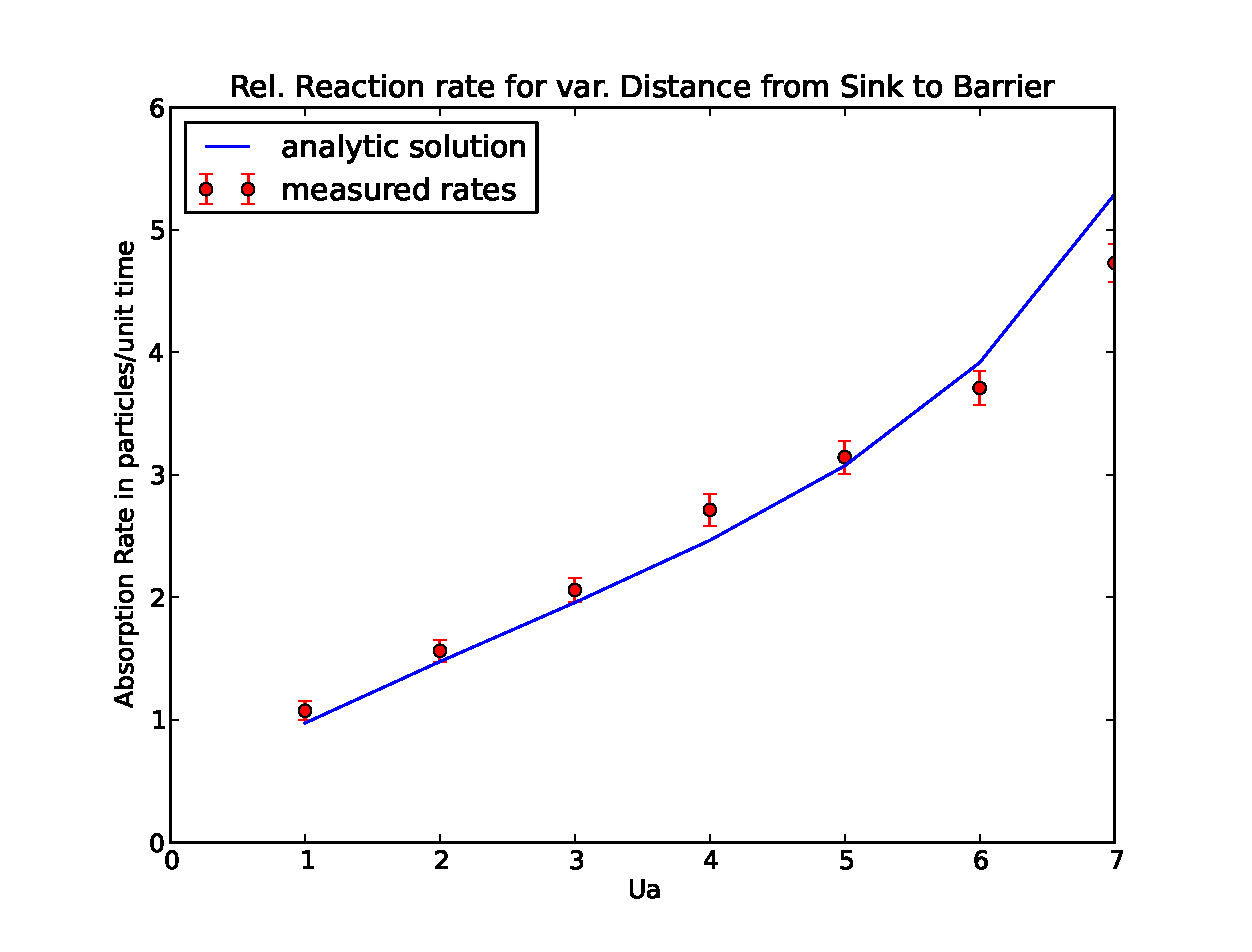
\includegraphics[width=.95 \textwidth, keepaspectratio]{plots/cp/ub/Kabs.eps}
%\end{minipage}\begin{minipage}{.5 \textwidth}
%    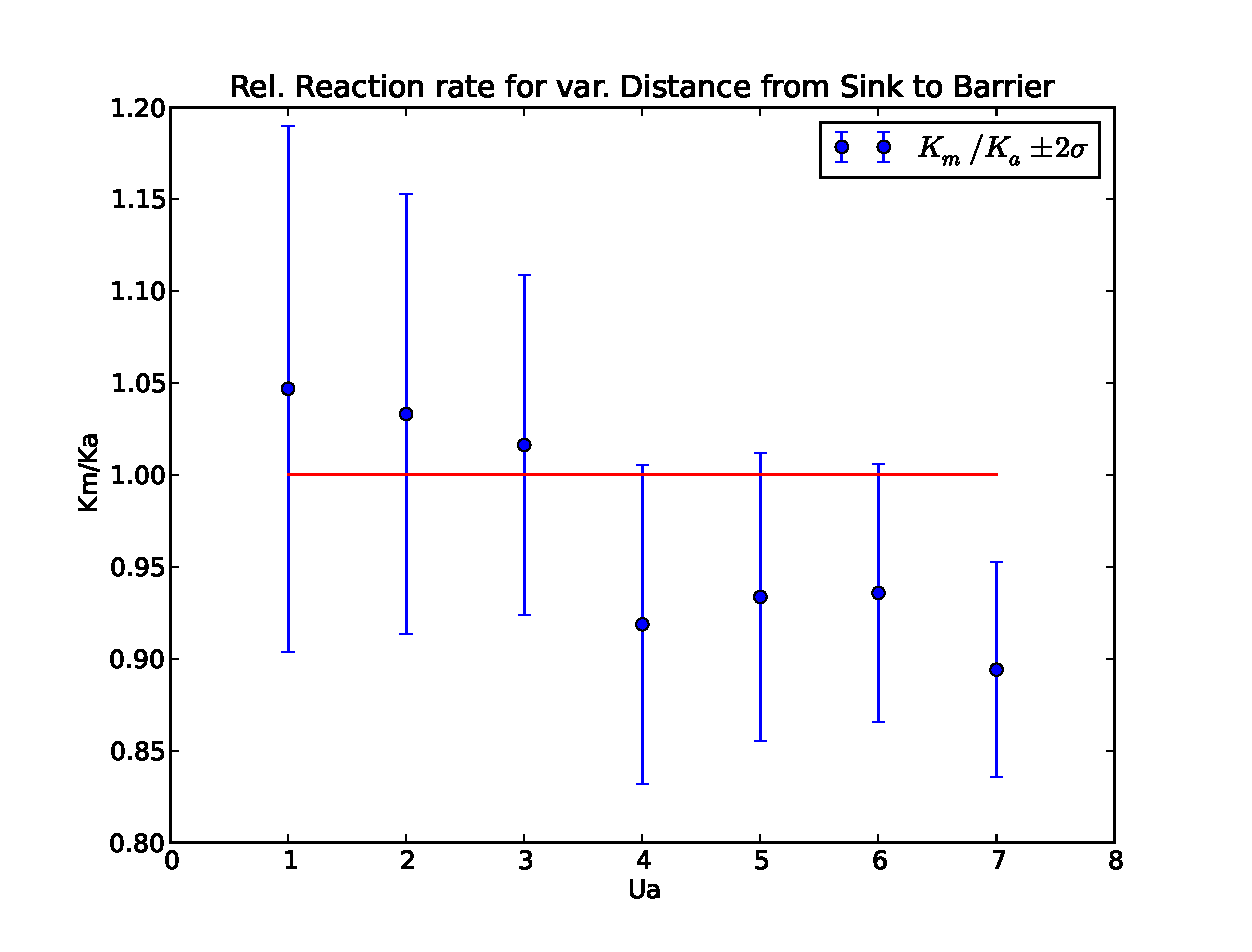
\includegraphics[width=.95 \textwidth, keepaspectratio]{plots/cp/ub/Krel.eps}
%\end{minipage}
%\caption{Absolute and relative Absorption rate for varying $U_b$}
%\label{fig:KUbCp}
%\end{figure}



\begin{appendices}
    \section{Code}
    \subsection{Main Program}
    \lstinputlisting{../BDS/BDS.f90}
    \subsection{Initialization and Initial conditions}
    \lstinputlisting{../BDS/init.f90}
    \subsection{Equations of Motion and Boundary Conditions}
    \lstinputlisting{../BDS/push.f90}
    \subsection{Variable calculation and I/O}
    \lstinputlisting{../BDS/statistics.f90}
    \subsection{Box averages, Jackknife Binning and Auto Correlation Correction}
    \lstinputlisting{../BDS/stat5.f90}
\end{appendices}

\end{document}
